\documentclass{article}
\usepackage{amsmath} % for the Dirac slash notation
\usepackage{slashed} % for the Dirac slash notation
\usepackage{graphicx} %for the images
\usepackage{amstext} % for \text macro mathmode in the table
\usepackage{array} % align elements in a table
\usepackage{physics}% bra ket notation
\usepackage{flexisym}% prime notation
\newcolumntype{P}[1]{>{\centering\arraybackslash}p{#1}} % verticle alignment of elements in a table
\newcolumntype{M}[1]{>{\centering\arraybackslash}m{#1}} % verticle and horizontal alignment of elements in a table
\usepackage{eufrak}
\usepackage{mathtools}
\usepackage{color}   % for coloring text
\usepackage{indentfirst} % indent first paragaraph of a section

\newcommand{\beq}{\begin{equation}}
\newcommand{\eeq}{\end{equation}}
\newcommand{\bea}{\begin{eqnarray}}
\newcommand{\eea}{\end{eqnarray}}
\newcommand{\pr}{\textprime}


\def\red{\color{red}}
\def\blue{\color{blue}}


\begin{document}
\centerline{\sc \LARGE Chiral Perturbation Theory}
\vspace{.5pc}
\centerline{\it Dulitha Jayakodige} 
\vspace{2pc}

\section {Introduction}


Chiral Perturbation Theory (ChPT) is an Effective Field Theory (EFT) that can be used to describe low energy properties of the strong interaction. According to the standard model Quantum Chromodynamics (QCD) the theory of quarks and gluons describes the strong interaction. Since QCD has asymptotic freedom at high energies, it can be analyzed using perturbative techniques. At low energies it's not possible because the larger coupling constant gives non convergent perturbative series expansions. Therefore non-perturbative methods are required to analyze QCD at low energies. Effective field theories and Lattice QCD are well established non-perturbative methods for the low energy end of the spectrum. ChPT is an EFT which is constructed with the Lagrangian consists with the chiral symmetry of QCD.



At low energies, confinement of quarks and gluons make composite particles and the interactions are stronger due to large coupling constant. At high energies, quarks and gluon interactions are weak due to small coupling constant. 




% QCD and χPT, are not written in terms of the same fields.
%The QCD Lagrangian has quark and gluon fields, whereas χPT has meson and baryon fields.


%The expansion parameter of χPT is p/Λχ, where Λχ ∼ 1 GeV is referred to as the scale of chiral symmetry breaking




\newpage
\section{Spontaneous Symmetry Breaking and \\ Goldstone Bosons}

Spontaneous Symmetry breaking is an underling concept of elementary particle physics and many other ares in physics such as superconductivity and ferromagnetism. 

Let's assume quarks don't have masses. Then the QCD lagrangian has the perfect chiral symmetry and it also undergoes spontaneous symmetry breaking, which gives us massless Goldstone bosons. Then the pions will not have masses. In reality quarks do have very small masses, therefore the chiral symmetry is not exact. CQD lagrangian undergoes explicit symmetry breaking which gives us non zero masses to pions. 

QCD is gauge theory which has continuous U(1) symmetry. QCD lagrangian has perfect chiral symmetry if the quarks don't have masses. In reality quarks have very small masses, therefore the chiral symmetry is not exact.

 


\newpage
\section{Lowest order Chiral Lagrangian}
To lowest order (minimum number of derivatives), the effective chiral Lagrangian:



$$\mathcal L_{2}=\frac{F^{2}}{4} \Big \langle \partial_{\mu} U^{\dag} \partial^{\mu} U \Big \rangle $$ \cite{pich1995chiral}. (page100)

Where, $\ U = exp(i \Phi/F) $, $ \Phi = \lambda^{a} \phi^{a}$ ,(when defining pion nucleon lagrangian,we will see u which is the square roof of this U) and  $ \lambda$'s are Gell-Mann matrices. \cite{scherer2003introduction} (page70)  $ F \approx 93.2 MeV$ pion decay constant \cite{pich1995chiral}. (page103)

$$ \Phi = \sqrt{2}  \left[
\begin{array}{ccc}
\frac{\pi^{0}}{\sqrt{2}} +\frac{\eta_{8}}{\sqrt{6}} & \pi^{+} & K^{+} \\
\pi^{-} & \frac{-\pi^{0}}{\sqrt{2}}+\frac{\eta_{8}}{\sqrt{6}} & K^{0}\\
K^{-} & \bar{K}^{0} & \frac{-2 \eta_{8}}{\sqrt{6}}
\end{array}
\right] $$ \cite{scherer2003introduction} (page70) ( also see My Calculation "Gell Mann Matrices") 

\vspace{10mm}
The Lagrangian can be simplified to (see my calculations "chiral lagrangian derivations")

$$\mathcal L_{2}=\frac{1}{4} \Big \langle \partial_{\mu} \Phi \partial^{\mu} \Phi \Big \rangle 
+\frac{1}{48F^{2}} \Big \langle \left[ \partial_{\mu}\Phi, \Phi \right] \left[ \partial^{\mu}\Phi, \Phi \right] \Big \rangle 
+ \mathcal{O} \left( \frac{1}{F^{4}} \right) $$

The first term can be simplified to,\cite{scherer2003introduction} (page71)
$$\mathcal L_{2}=\frac{1}{2}  \partial_{\mu} \phi \partial^{\mu} \phi  
+ \mathcal{O} \left( \frac{1}{F^{2}} \right) $$ 

The second term can be expressed with structure constants of SU3(see my calculations "chiral lagrangian derivations")
$$\Big \langle \left[ \partial_{\mu}\Phi, \Phi \right] \left[ \partial^{\mu}\Phi, \Phi \right] \Big \rangle =
-8 \partial_{\mu} \phi^{a} \phi^{b} \partial^{\mu} \phi^{c} \phi^{d} f^{abe}  f^{cde}$$
Where $ f^{abc} =\frac{1}{4i} \langle \left[ \lambda^{a} \lambda^{b}\right] \lambda^{c}\rangle$, \cite{scherer2003introduction} (page 03)







\newpage
\section{Mass Term}
Lagrangian with the mass term can be written with the unknown factor B \cite{kubis2007introduction} (page 09) (B is related to the chiral quark condensate Ref: Sherere pg74)
$$\mathcal L_{2}=\frac{F^{2}}{4} \Big \langle \partial_{\mu} U \partial^{\mu} U^{\dag} \Big \rangle 
+\frac{F^{2}}{2} B \Big \langle \mathcal M \left( U + U^{\dag} \right) \Big \rangle$$

where quark mass matrix $ \mathcal M =  \left[ \begin{array}{ccc}
	m_{u} & 0 & 0 \\
	0 & m_{d} & 0\\
	0 & 0 & m_{s} \end{array} \right] $
\
This mass therm is due to symmetry breaking \cite{scherer2003introduction} (page74)
$$	\mathcal L_{s.b} =\frac{F^{2}}{2} B \Big \langle \mathcal M \left( U + U^{\dag} \right) \Big \rangle =
 \frac{F^{2}B}{2} \Big \langle \mathcal M \left( 2- \frac{\Phi^{2}}{F^{2}} + \frac{\Phi^{4}}{12F^{4}}+...\right) \Big \rangle $$
 
"In order to determine the masses of the Goldstone bosons, we identify the terms of second order in the fields in $	\mathcal L_{s.b}$ \cite{scherer2003introduction} (page74)" 
 
$$	\mathcal L_{s.b} = \frac{B}{2} \Big \langle \mathcal M \left( \Phi^{2}\right) \Big \rangle +... $$
\begin{eqnarray*}
	\mathcal L_{s.b} & = & 
	\frac{B}{2} \{ 2(m_{u}+m_{d}) \pi^{+}\pi^{-} + 2(m_{u}+m_{s}) K^{+}K^{-} + 2(m_{d}+m_{s})K_{0}\bar{K}_{0} \\& & 
	+ (m_{u}+m_{d}) \pi^{0}\pi^{0} +\frac{2}{\sqrt{3}}(m_{u}-m_{d}) \pi^{0} \eta  +\frac{1}{3}(m_{u}+m_{d}+4m_{s}) \eta\eta
\end{eqnarray*}
\cite{scherer2003introduction} (page 03) (see Mathematica calculations "Gell Mann Oakes Relations")
\
Gell-Mann, Oakes, and Renner relations, $ M^{2}_{GB} \propto m_{q}  $ can be derived (see my calculations "chiral lagrangian derivations")\cite{kubis2007introduction} (page 10)

\begin{eqnarray*}
	M^{2}_{\pi^{\pm}} & = &  \frac{B}{2} (m_{u}+m_{d}) \\
	M^{2}_{K^{\pm}} & = &  \frac{B}{2} (m_{u}+m_{s}) \\
	M^{2}_{K_{0}^{\pm}} & = &  \frac{B}{2} (m_{d}+m_{s}) \\
\end{eqnarray*}

Quark mass rations can be calculated using above relations as \cite{kubis2007introduction} (page 10)
\begin{eqnarray*}
	\frac{m_{u}}{m_{d}} & = &  0.66 \\
	\frac{m_{s}}{m_{d}} & = &  22 \\
\end{eqnarray*}








\newpage

The coupling of the Lagrangian to external vector $ v_{\mu} $ and axial vector $ a_{\mu} $ can be done by replacing the ordinary derivative by a
covariant derivative. \cite{kubis2007introduction} (page 11)

$$ \partial_{\mu} U  \rightarrow  D_{\mu} U = \partial_{\mu} U -ir_{\mu}U +iUl_{\mu} $$ \cite{scherer2003introduction} (page 80)

$$ D_{\mu} U = \partial_{\mu} U -i \left[v_{\mu},U\right]  -i \{a_{\mu},U \}$$ \cite{kubis2007introduction} (page 11)


\vspace{10mm}
The most general, locally invariant, effective Lagrangian at lowest chiral order

$$\mathcal L_{2}=\frac{F^{2}}{4} \Big \langle D_{\mu} U (D^{\mu} U)^{\dag} \Big \rangle 
+\frac{F^{2}}{4} \Big \langle   \chi U^{\dag}  +U \chi ^{\dag} \Big \rangle$$
\cite{scherer2003introduction} (page 82)

Where $ \chi $ , is a linear combination of a scalar and pseudoscalar $ \chi = 2B(s+ip)$ \cite{scherer2003introduction} (page 80)
In SU(2) $\chi = 2B M = 2B \left[ \begin{array}{cc}
	m & 0 \\
	0 & m\end{array} \right] $ \cite{scherer2003introduction} (page 88)

\vspace{5mm}	
At $\mathcal{O}(p^2)$, $ M_{\pi}^2= 2Bm $ \cite{scherer2003introduction} (page 83)	

$$\mathcal L_{2}=\frac{F^{2}}{4} \Big \langle D_{\mu} U (D^{\mu} U)^{\dag} \Big \rangle 
+\frac{F^{2}}{4} M_{\pi}^2 \Big \langle  U^{\dag}  +U  \Big \rangle$$

This can be simplified as follows, 

$$\mathcal L_{2}=\frac{1}{4} \Big \langle \partial_{\mu} \Phi \partial^{\mu} \Phi \Big \rangle 
+\frac{1}{48F^{2}} \Big \langle \left[ \partial_{\mu}\Phi, \Phi \right] \left[ \partial^{\mu}\Phi, \Phi \right] \Big \rangle + \frac{F^{2}M_{\pi}^2}{4} \Big \langle  2- \frac{\Phi^{2}}{F^{2}} + \frac{\Phi^{4}}{12F^{4}} \Big \rangle $$

$$\mathcal L_{2}=\frac{1}{4} \Big \langle \partial_{\mu} \Phi \partial^{\mu} \Phi \Big \rangle 
+ \frac{F^{2}M_{\pi}^2}{2} 
+ \frac{F^{2}M_{\pi}^2}{4} \langle  \Phi^{2}  \rangle 
+\frac{1}{48F^{2}} \left( \Big \langle \left[ \partial_{\mu}\Phi, \Phi \right] \left[ \partial^{\mu}\Phi, \Phi \right] \Big \rangle 
+M_{\pi}^2  \langle \Phi^{4}  \rangle \right)$$


\newpage
\section{The Chiral Lagrangian at Fourth Order}


$$\mathcal L_{4}=L_{1} \Big \langle D_{\mu} U (D^{\mu} U)^{\dag} \Big \rangle 
+$$



\cite{scherer2003introduction} (page 93)
\cite{pich1995chiral}. (page106)










\newpage
\section{Baryonic Effective Lagrangian ( remove)   }


The most general Lagrangian with the smallest number of derivatives is given by

$$ \mathcal{L}_{\pi,N}^{(1)} = \bar{\Psi} \left( i\slashed{D} -\mathring{m}_{N}  + \frac{\mathring{g}_{A}}{2} \gamma^{\mu} \gamma_{5} u_{\mu} \right) \Psi$$ 

Where $\mathring{m}_{N}= 883 MeV$ and $\mathring{g}_{A}= 1.267 MeV$ \cite{scherer2003introduction} (page 122)

\vspace{5mm}
With external sources $ r_{\mu}$ , $ l_{\mu}$, and $v_{\mu}^{(s)} $ \cite{scherer2003introduction} (page 121,122)

$$ D_{\mu} = \partial_{\mu} + \Gamma_{\mu} -iv_{\mu}^{(s)}$$
$$ \Gamma_{\mu} = \frac{1}{2} \left[  u^{\dag} (\partial_{\mu}-ir_{\mu}) u + u (\partial_{\mu}-il_{\mu} ) u^{\dag} \right] $$
$$ u_{\mu} = i \left[  u^{\dag} (\partial_{\mu}-ir_{\mu}) u - u (\partial_{\mu}-il_{\mu} ) u^{\dag} \right]   $$

Here, $u^{2}= U = exp(i \Phi/F) $, $ \Phi = \tau^{a} \phi^{a} $

\vspace{5mm}

Without external sources, $ r_{\mu} = l_{\mu} =0 $, and $v_{\mu}^{(s)}=0 $ \cite{scherer2003introduction} (page 123)
$ D_{\mu} = \partial_{\mu} + T_{\mu}$ ,  
$\Gamma_{\mu} = \frac{1}{2} \left(  u^{\dag} \partial_{\mu} u + u \partial_{\mu} u^{\dag} \right)   $, and
$ u_{\mu} = i \left(  u^{\dag} \partial_{\mu} u - u \partial_{\mu} u^{\dag} \right)   $
Baryonic Effective Lagrangian


$$ \mathcal{L}_{\pi,N}^{(1)} = \bar{\Psi} \left( i\gamma^{\mu} \left(  \partial_{\mu} + \frac{1}{2} \left(  u^{\dag} \partial_{\mu} u + u \partial_{\mu} u^{\dag} \right)  \right) 
-\mathring{m}_{N}  
+ i \frac{\mathring{g}_{A}}{2} \gamma^{\mu} \gamma_{5} \left(  u^{\dag} \partial_{\mu} u - u \partial_{\mu} u^{\dag} \right) \right) \Psi$$ 

(see my calculations "Baryonic Effective Lagrangian")

\vspace{10mm}
Interaction Lagrangian containing one and two pion fields

$$ \mathcal{L}_{\pi,N}^{(1)} = \bar{\Psi} \left( i\gamma^{\mu} \left(  \partial_{\mu} + i \frac{\epsilon_{abc}}{4F^{2}} \phi^{a} \partial_{\mu} \phi^{b} \sigma_{c} \right) 
-\mathring{m}_{N}  
- \frac{\mathring{g}_{A}}{2} \gamma^{\mu} \gamma_{5}  \partial_{\mu} \phi^{d} \sigma_{d} \right) \Psi$$
(see my calculations "Baryonic Effective Lagrangian")

\vspace{10mm}
Pion-nucleon interaction Lagrangian
$$ \mathcal{L}_{int} = -\frac{\epsilon_{abc}}{4F^{2}}\bar{\Psi} \gamma^{5} \phi^{a} \partial_{\mu} \phi^{b} \sigma_{c} 
- \frac{\mathring{g}_{A}}{2} \bar{\Psi} \gamma^{\mu} \gamma_{5}  \partial_{\mu} \phi^{a} \sigma_{a} \Psi
$$

Here, the first term corresponds to interaction of two pion field  with the nucleon at a single point and the second therm is the pseudovector pion-nucleon coupling. \cite{scherer2003introduction} (page 134)


\newpage

\section{Realtivisic Pion Nucleon Lagrangian}

$$ \mathcal{L}_{\pi,N}^{(1)} = \bar{\Psi} \left( i\slashed{D} -\mathring{m}_{N}  + \frac{\mathring{g}_{A}}{2} \gamma^{\mu} \gamma_{5} u_{\mu} \right) \Psi$$ 

Where $\mathring{m}_{N}= 883 MeV$ and $\mathring{g}_{A}= 1.267 MeV$ \cite{scherer2003introduction} (page 122)

\vspace{5mm}
With external sources $ r_{\mu}$ , $ l_{\mu}$, and $v_{\mu}^{(s)} $ \cite{scherer2003introduction} (page 121,122)

$$ D_{\mu} = \partial_{\mu} + \Gamma_{\mu} -iv_{\mu}^{(s)}$$
$$ \Gamma_{\mu} = \frac{1}{2} \left[  u^{\dag} (\partial_{\mu}-ir_{\mu}) u + u (\partial_{\mu}-il_{\mu} ) u^{\dag} \right] $$
$$ u_{\mu} = i \left[  u^{\dag} (\partial_{\mu}-ir_{\mu}) u - u (\partial_{\mu}-il_{\mu} ) u^{\dag} \right]   $$

\vspace{5mm}


Without external sources, $ r_{\mu} = l_{\mu} =0 $, and $v_{\mu}^{(s)}=0 $ \cite{scherer2003introduction} (page 123)
$ D_{\mu} = \partial_{\mu} + T_{\mu}$ ,  
$\Gamma_{\mu} = \frac{1}{2} \left(  u^{\dag} \partial_{\mu} u + u \partial_{\mu} u^{\dag} \right)   $, and
$ u_{\mu} = i \left(  u^{\dag} \partial_{\mu} u - u \partial_{\mu} u^{\dag} \right)   $


\vspace{5mm}
Baryonic Effective Lagrangian
$$ \mathcal{L}_{\pi,N}^{(1)} = \bar{\Psi} \left( i\gamma^{\mu}  \partial_{\mu}    -\mathring{m}_{N}
 + i\frac{\gamma^{\mu}}{2} \left(  u^{\dag} \partial_{\mu} u + u \partial_{\mu} u^{\dag}  \right)  
+ i \frac{\mathring{g}_{A}}{2} \gamma^{\mu} \gamma_{5} \left(  u^{\dag} \partial_{\mu} u - u \partial_{\mu} u^{\dag} \right) \right) \Psi$$ 

\vspace{5mm}
Here, $u^{2}= U = exp(i \Pi/F) $, $ \Pi = \tau^{a} \pi^{a} $


 
Using following approximations (pi here should be big Pi,this is a mistake,correct it)

$$ \left(  u^{\dag} \partial_{\mu} u + u \partial_{\mu} u^{\dag} \right) = 
2\left( \frac{ \left[\pi,\partial_{\mu}\pi \right] }{8F^2} 
+ \frac{ \left[\left[\left[\partial_{\mu}\pi,\pi \right],\pi \right],\pi \right] }{384F^4} +... \right) $$

$$ \left(  u^{\dag} \partial_{\mu} u - u \partial_{\mu} u^{\dag} \right) = -i
\left( \frac{ -\partial_{\mu}\pi }{F} 
+ \frac{ \left[\left[\partial_{\mu}\pi,\pi \right],\pi \right] }{24F^3} +... \right) $$



Baryonic Effective Lagrangian (pi here should be big Pi,this is a mistake,correct it)
$$ \mathcal{L}_{\pi,N}^{(1)} = \bar{\Psi} \left( i\gamma^{\mu}  \partial_{\mu}    -\mathring{m}_{N}
- \frac{\mathring{g}_{A} \gamma^{\mu} \gamma_{5} \partial_{\mu}\pi}{2F} 
+ \frac{i\gamma^{\mu} \left[\pi,\partial_{\mu}\pi \right] }{8F^2}  
+ \frac{\mathring{g}_{A} \gamma^{\mu} \gamma_{5} \left[\left[\partial_{\mu}\pi,\pi \right],\pi \right]}{48F^3}
+ \frac{i\gamma^{\mu} \left[\left[\left[\partial_{\mu}\pi,\pi \right],\pi \right],\pi \right] }{384F^4}  
+... \right) \Psi$$ 





\newpage
\section{Relativistic Feynman Rules}


\begin{table}
	[ht] \caption{Feynman Rules} 
	\vspace{5mm}
	\begin{tabular}{ M{5.5cm} M{5.5cm}}
		\hline 
		Graph Element & Mathematical Equivalent \\
		\hline
		\includegraphics[trim={7cm 23cm 7cm 2cm}, clip=true,width=
		5cm]{images/single_pion_vertex.eps} & $ \frac{\mathring{g}_{A}}{2F} \slashed k \gamma_{5}  \tau^{a}$   \\ %trim={<left> <lower> <right> <upper>}
		\includegraphics[trim={7cm 23cm 7cm 2cm}, clip=true,width=
		5cm]{images/single_pion_vertex.eps} & $ \frac{\left(\slashed k_1 +\slashed k_2 \right)}{4F^2}  \epsilon_{abc}  \tau^{c}$   \\ %trim={<left> <lower> <right> <upper>}
		\includegraphics[trim={7cm 23cm 7cm 2cm}, clip=true,width= 4cm]{images/baryon_propagator.eps} & $ \frac{i}{11111} $ \\
		\includegraphics[trim={7cm 23cm 7cm 2cm}, clip=true,width= 4cm]{images/meson_propargator.eps} & $ \frac{i}{1111} $ \\
		\hline
	\end{tabular}
\end{table}







\newpage
\section{HBChPT form Relativistic L , by approximations}


\begin{table}
	[ht] \caption{Feynman Rules} 
	\vspace{5mm}
	\begin{tabular}{ M{5.5cm} M{5.5cm}}
		\hline 
		Graph Element & Mathematical Equivalent \\
		\hline 
		\includegraphics[trim={7cm 23cm 7cm 2cm}, clip=true,width= 		 5cm]{images/single_pion_vertex.eps} & $ -\frac{\mathring{g}_{A}}{F_{\pi}}  k^{i}G^{ia}$ here  $G^{ia}=\frac{\tau^i \tau^a}{2}$ \\ %trim={<left> <lower> <right> <upper>}
		\includegraphics[trim={7cm 23cm 7cm 2cm}, clip=true,width=
		5cm]{images/single_pion_vertex.eps} & $ \frac{\left(\slashed k^0_1 +\slashed k^0_2 \right)}{2F^2}  \epsilon_{abc}  I^{c}$ here  $I^{c}=\frac{\tau^c}{2}$  \\ %trim={<left> <lower> <right> <upper>}
		\includegraphics[trim={7cm 23cm 7cm 2cm}, clip=true,width= 4cm]{images/baryon_propagator.eps} & $ \frac{iP_{n}}{p^{0}- \delta m_{n}+ i \epsilon} $ \\
		\includegraphics[trim={7cm 23cm 7cm 2cm}, clip=true,width= 4cm]{images/meson_propargator.eps} & $ \frac{i}{k^{2}-M_{\pi}^{2}  +i\epsilon} $ \\
		\hline
	\end{tabular}
\end{table}


\newpage
\section{HBChPT and 1/Nc Lagrangian}

In the $\xi $ expansion, the Lagrangian for the combined HBChPT and 1/Nc expansions to order $\xi$

$$ \mathcal{L}_{B}^{(1)} = B^{\dag} \left( iD_0 + \mathring{g}_A u^{ia} G^{ia} -\frac{C_{HF}}{N_c} \hat{S}^2 +\frac{c_1}{2 \Lambda } \hat{\chi}_+ \right) B $$ 

\cite{Fernando2018} \cite{Fernando2020} \cite{Cordon2013}

The chiral covariant derivative $ D_{\mu} = \partial_{\mu} -i \Gamma_{\mu}$
$$ \Gamma_{\mu} = \frac{1}{2} \left[  u^{\dag} (i\partial_{\mu} +r_{\mu}) u + u (i\partial_{\mu}+l_{\mu} ) u^{\dag} \right] $$

Without external sources, gauge sources become zero $ r_{\mu} = l_{\mu} =0 $, therefore, $D_{0} =\partial_{0}+ \frac{1}{2} \left(  u^{\dag} \partial_{0} u + u \partial_{0} u^{\dag} \right)   $, 

\vspace{5mm}
axial Maurer-Cartan
$$ u_{\mu} = \left[  u^{\dag} (i\partial_{\mu} +r_{\mu}) u - u (i\partial_{\mu}+l_{\mu} ) u^{\dag} \right]   $$

Without external sources, gauge sources become zero $ r_{\mu} = l_{\mu} =0 $, therefore, $u_i =i \left(  u^{\dag} \partial_{i} u - u \partial_{i} u^{\dag} \right)   $and  $u^i =i \left(  u^{\dag} \partial^{i} u - u \partial^{i} u^{\dag} \right)   $.

\vspace{5mm}
According to \cite{CalleCordon2014} 
$$ u^{ia} = \frac{1}{2} \left< u^i \tau ^a \right> $$

\vspace{5mm}
Here we use, $u^{2}= U = exp(i \Pi/F) $, $ \Pi = \tau^{a} \pi^{a} $


Approximations

$$ \left(  u^{\dag} \partial_0 u + u \partial_0 u^{\dag} \right) = 
2\left( \frac{ \left[\Pi,\partial_0\Pi \right] }{8F^2} 
+ \frac{ \left[\left[\left[\partial_0\Pi,\Pi \right],\Pi \right],\Pi \right] }{384F^4} +... \right) $$

$$ \left(  u^{\dag} \partial^i u - u \partial^i u^{\dag} \right) = -i
\left( \frac{ -\partial^i \Pi }{F} 
+ \frac{ \left[\left[\partial^i\Pi,\Pi \right],\Pi \right] }{24F^3} +... \right) $$


\vspace{5mm}
Leading order terms of the Lagrangian can be written as fallows.(see my calculations "Feynman Rules from Non relativistic L") 

\bea
\mathcal{L}_{B}^{(1)} \approx B^{\dag} \left( i\partial
+\frac{\mathring{g}_A}{2} \frac{ \left< -\partial^i\Pi\tau^a \right> }{F}  G^{ia} 
+ i\frac{ \left[\Pi,\partial_0 \Pi \right] }{8F^2} 
+\frac{\mathring{g}_A}{2} \frac{ \left<  \left[\left[\partial^i\Pi,\Pi \right],\Pi \right] \tau^a \right>  }{24F^3}  G^{ia}  
\right.
\nonumber\\
\left.
+i\frac{ \left[\left[\left[\partial_0\Pi,\Pi \right],\Pi \right],\Pi \right] }{384F^4}
-\frac{C_{HF}}{N_c} \hat{S}^2 +\frac{c_1}{2 \Lambda } \hat{\chi}_+ \right) B
\nonumber
\eea


Where $ \chi $ , is a linear combination of a scalar and pseudoscalar \cite{Fernando2018} $ \chi = 2B_0 (s+ip)$ In SU(2) $\chi = 2B_0 M = 2B_0 \left[ \begin{array}{cc}
m & 0 \\
0 & m\end{array} \right] $ \cite{scherer2003introduction} (page 88)



$ \chi_{\pm}  = u^{\dagger} \chi u^{\dagger} \pm u \chi^{\dagger} u $ 

$ \chi_{\pm}^{0} =\left\langle\chi_{\pm}\right\rangle $

$  \chi_{\pm}^{a}  = \left\langle\chi_{\pm} I^a\right\rangle   $

$ \tilde{\chi}_{\pm} = \chi_{\pm}^{a} I^{a} $

\vspace{5mm}

$ \hat{\chi}_{+} = \tilde{\chi}_{+} + N_c \: \chi_{+}^{0} $

For convenience, a scale $ \Lambda $ is introduced, which can be chosen to be a typical QCD scale, in order to render most of the LECs dimensionless. In the calculations,$ \Lambda = m_\rho $ will be chosen.\cite{Fernando2018}

$C_{HF}$ is equal to hyperfine splitting $C_{HF} = M_\Delta -M_N $ 

\newpage
\section{Feynman Rules}

Vertices are given by:  $i \; (factors \;in \; \mathcal{L})$. Outgoing Pion gives $ik$ for $\partial \Pi$. These Feynman Rules can be used to get get $i \mathcal{M}$

\begin{table}
	[ht] \caption{Feynman Rules for Vertices} 
	\vspace{5mm}
	\begin{tabular}{ M{4cm} M{4.5cm} M{4.5cm}}
		\hline 
		Graph Element & Interaction Lagrangian & Feynman Rule\\
		\hline 
		\includegraphics[trim={7cm 24cm 7cm 2cm}, clip=true,width=  4cm]{images/Pi_N_FR_one.eps} &		
		 $B^{\dag}  \frac{\mathring{g}_A}{2} \frac{ \left< -\partial^i\Pi\tau^a \right> }{F}  G^{ia}  B $&
		 $ \frac{\mathring{g}_{A}}{F}  k^{i}G^{ia} $  \\ 
		\includegraphics[trim={7cm 24cm 7cm 2cm}, clip=true,width= 	4cm]{images/Pi_N_FR_two.eps} &
		 $B^{\dag} i\frac{ \left[\Pi,\partial_0 \Pi \right] }{8F^2} B $ &
		 $\frac{\left( k^0_2 - k^0_1 \right)}{2F^2}  \epsilon_{abc}  I^{c}$ \\ 
		\includegraphics[trim={7cm 24cm 7cm 2cm}, clip=true,width= 4cm]{images/Pi_N_FR_three.eps} &
		 $B^{\dag} \frac{\mathring{g}_A}{2} \frac{ \left<  \left[\left[\partial^i\Pi,\Pi \right],\Pi \right] \tau^a \right>  }{24F^3}  G^{ia} B $&
		        \\
		\includegraphics[trim={7cm 24cm 7cm 2cm}, clip=true,width= 4cm]{images/Pi_N_FR_four.eps} &
		 $B^{\dag} i\frac{ \left[\left[\left[\partial_0\Pi,\Pi \right],\Pi \right],\Pi \right] }{384F^4} B $&
		        \\
		\includegraphics[trim={7cm 24cm 7cm 2cm}, clip=true,width= 4cm]{images/Pi_N_FR_pion.eps} &
		 $ \frac{1}{48F^{2}} \left( \Big \langle \left[ \partial_{\mu}\Pi, \Pi \right] \left[ \partial^{\mu}\Pi, \Pi \right] \Big \rangle 
		 +M_{\pi}^2  \langle \Pi^{4}  \rangle \right)$&
		        \\
		\hline
	\end{tabular}
\end{table}

Here  $G^{ia}=\frac{\tau^i \tau^a}{2}$, $I^{c}=\frac{\tau^c}{2}$ \\
with $ \tau^a =\begin{Bmatrix} \begin{pmatrix}0&1\\1&0\end{pmatrix}, & \begin{pmatrix}0&-i\\i&0\end{pmatrix}, & \begin{pmatrix}1&0\\0&-1\end{pmatrix} \end{Bmatrix}   $ 

\newpage
\begin{table}
	[ht]
	\centering
	\caption{Feynman Rules for Propagators} 
	\vspace{5mm}
	\begin{tabular}{ M{3.5cm} M{3.5cm}}
		\hline 
		Graph Element & Feynman Rule\\
		\hline 
		\includegraphics[trim={7cm 25cm 7cm 2cm}, clip=true,width=  4cm]{images/Pi_N_FR_fermion.eps} &		
		$\frac{i}{p^0-\delta m_n+i\epsilon}$\\ 
		\includegraphics[trim={7cm 25cm 7cm 2cm}, clip=true,width= 	4cm]{images/Pi_N_FR_meson.eps} &
		$ \frac{i}{k^2-M^2+i\epsilon}$  \\ 
		\hline
	\end{tabular}
\end{table}


\newpage
\section{Dimensional Regularization}


These integrals usually diverges. Therefore, its impossible to evaluate as a normal integration. There are very profound mathematical techniques to handle those divergences. \textbf{Dimensional Regularization} is used here to isolate the divergence of the integral.

introduced in 1972 by ‘t Hooft and Veltman (and by Bollini
and Gambiagi) as a method to regularise ultraviolet (UV) divergences in a gauge invariant way


The idea is to work in $D = 4 - 2/\epsilon$ spacetime dimensions. Divergences for D goes to 4 will thus
appear as poles in $1/\epsilon$

\newpage
\section{Feynman Parameters}

 Feynman Parameters is one of the most important mathematical technique which is used to simplify loop integrals. According to this technique, the denominator can be simplified by introducing extra integration with respect to an auxiliary variable. This allows to squeeze \textbf{n} number of denominators in to a single quadratic polynomial, raised to the power of \textbf{n}. Most general form of the Feynman Parameters is given by,\cite{Peskin1995}

\beq
\frac{1}{A_1A_2...A_n} =  \int_{0}^{1} d\alpha_1 \alpha_2...\alpha_n   \frac{\delta \left( \Sigma \alpha_i -1 \right) (n-1)!}{ \left[ \alpha_1 A_1+ \alpha_2 A_2 +...+ \alpha_n A_n \right] ^n }  
\eeq

\vspace{5mm}
For two denominators, it simplifies to
\beq
\frac{1}{AB} =  \int_{0}^{1} d\alpha   \frac{1}{ \left[ \alpha A+(1-\alpha) B \right] ^2 }  
\eeq

This formula is used when two meson propagators appears as the denominator. When a meson propagator and baryon propagator appears, following alternative form is used. It can be obtain using change of variable $\lambda=\alpha/(1-\alpha)$
\beq
\frac{1}{AB} =  \int_{0}^{\infty} d\lambda  \frac{1}{ \left[ A+\lambda B \right] ^2 } 
\eeq

Combination of these two forms is useful when the denominator has two meson propagators and a baryon propagator.
\beq
\frac{1}{ABC} =  \int_{0}^{1} d\alpha  \int_{0}^{\infty} d\lambda  \frac{2}{ \left[ \lambda A + \alpha B+(1-\alpha) C \right] ^3 }  
\eeq

After applying Feynman Parameters technique, the denominator simplifies to a quadratic polynomial. Therefore preforming d-dimension integral is much easier, but there are new integrals to evaluate. Some of those new integrals are difficult integrate, specially integrals over $\lambda$. They can be evaluated at the very end of the calculation. Following \textbf{Feynman parameter Integrals} are very useful for evaluating those $\lambda$ integrals.

 

\vspace{5mm}
Most general form of $\lambda$ integrals (J integrals) is following
\bea
J\left( \nu, n \right) \equiv &&J\left( c_0 , c_1, \lambda_0, d, \nu, n \right) 
\nonumber\\
=&&\int_{0}^{\infty} \left( \lambda-\lambda_0\right)^n \left[ c_0 + c_1 \left( \lambda-\lambda_0\right)^2   \right]^{d/2-\nu} d\lambda
\eea

\vspace{2mm}
Here $ J\left( \nu ,1 \right) $ can be calculated explicitly.

$$ J\left( \nu,1 \right) =  \frac{-\left( c_0 + c_1 \lambda_0^2 \right)^{d/2-\nu +1}}{2c_1 \left(d/2-\nu+1\right)}$$

\vspace{5mm}
$  J\left( 3,0 \right)$ can be calculated with $d=4-2\epsilon$
\bea
\left( 3,0 \right) =&& \frac{1}{\sqrt{c_0 c_1}} \left( \frac{\pi}{2} + arctan \left( \lambda_0 \sqrt{\frac{c_1}{c_0}}\right) \right)    - \epsilon \int_{0}^{\infty} \frac{ log \left( c_0 + c_1 \lambda_0^2 \right)}{\left( c_0 + c_1 \lambda_0^2   \right)}   d\lambda 
\nonumber\\
= &&J_{30}^0 +\epsilon J_{30}^1
\eea

Following recurrence relationships are useful to evaluate remaining integrals.

\beq 
 J\left( \nu,0 \right) = \frac{c_0 \left(d-2\nu \right)}{\left(d-2\nu+1\right)} J\left( \nu+1, 0\right) + \frac{\lambda_0 \left( c_0 + c_1 \lambda_0^2 \right)^{d/2-\nu}}{\left(d-2\nu+1\right)} 
\eeq

\beq 
J\left( \nu,n \right) = \frac{1}{c_1} \left( J\left( \nu-1,n-2 \right)-c_0 J\left( \nu,n-2 \right) \right) 
\eeq


\vspace{5mm}
Some commonly used J integrals are given below
\bea
		J\left( 2,0 \right) &&= \lambda_0 +\epsilon \left( \lambda_0 \left[ 2-log \left( c_0 + c_1 \lambda_0^2 \right)  \right] -2c_0 J_{30}^0 \right) + \mathcal{O} \left( \epsilon^2 \right)   \\
		J\left( 1,0 \right) &&= c_0 \lambda_0 + \frac{c_1 \lambda_0^3}{3}  \\
		&& +\epsilon \left(    \frac{-4c_0^2 J_{30}^0}{3}      +   \frac{c_1\lambda_0^3}{9} \left[ 2-3log \left( c_0 + c_1 \lambda_0^2 \right)  \right]     +     \frac{c_0\lambda_0}{3} \left[4-3log \left( c_0 + c_1 \lambda_0^2 \right)  \right]            \right) + \mathcal{O} \left( \epsilon^2 \right)	\nonumber\\
		J\left( 2,1 \right) &&= \frac{- \left( c_0 +c_1 \lambda_0^2 \right) }{2c_1} +\epsilon \frac{ \left( c_0 +c_1 \lambda_0^2 \right) }{2c_1} \left(  log \left( c_0 +c_1 \lambda_0^2 \right) -1 \right) + \mathcal{O} \left( \epsilon^2 \right) \\
		J\left( 2,2 \right) &&=  \frac{\lambda_0^3}{3} 
		+\epsilon \left(    \frac{2c_0^2 J_{30}^0}{3c_1}   -\frac{2c_0 \lambda_0 }{3c_1}      + \frac{\lambda_0^3}{9} \left[ 2-3log \left( c_0 + c_1 \lambda_0^2 \right)  \right]         \right) + \mathcal{O} \left( \epsilon^2 \right)	
\eea


\newpage
\section{Loop Integrals}


Loop integrals appear, when calculating Feynman diagrams with loops. They are 4-dimensional integral over the four momentum of a virtual particle. Depending on the diagram, couple of different types on integrals appear. They were categorized based on their denominator.

\subsection{Types of Loop Integrals}

\subsubsection{H integral}

\begin{figure}[h]
\caption{single meson loop}
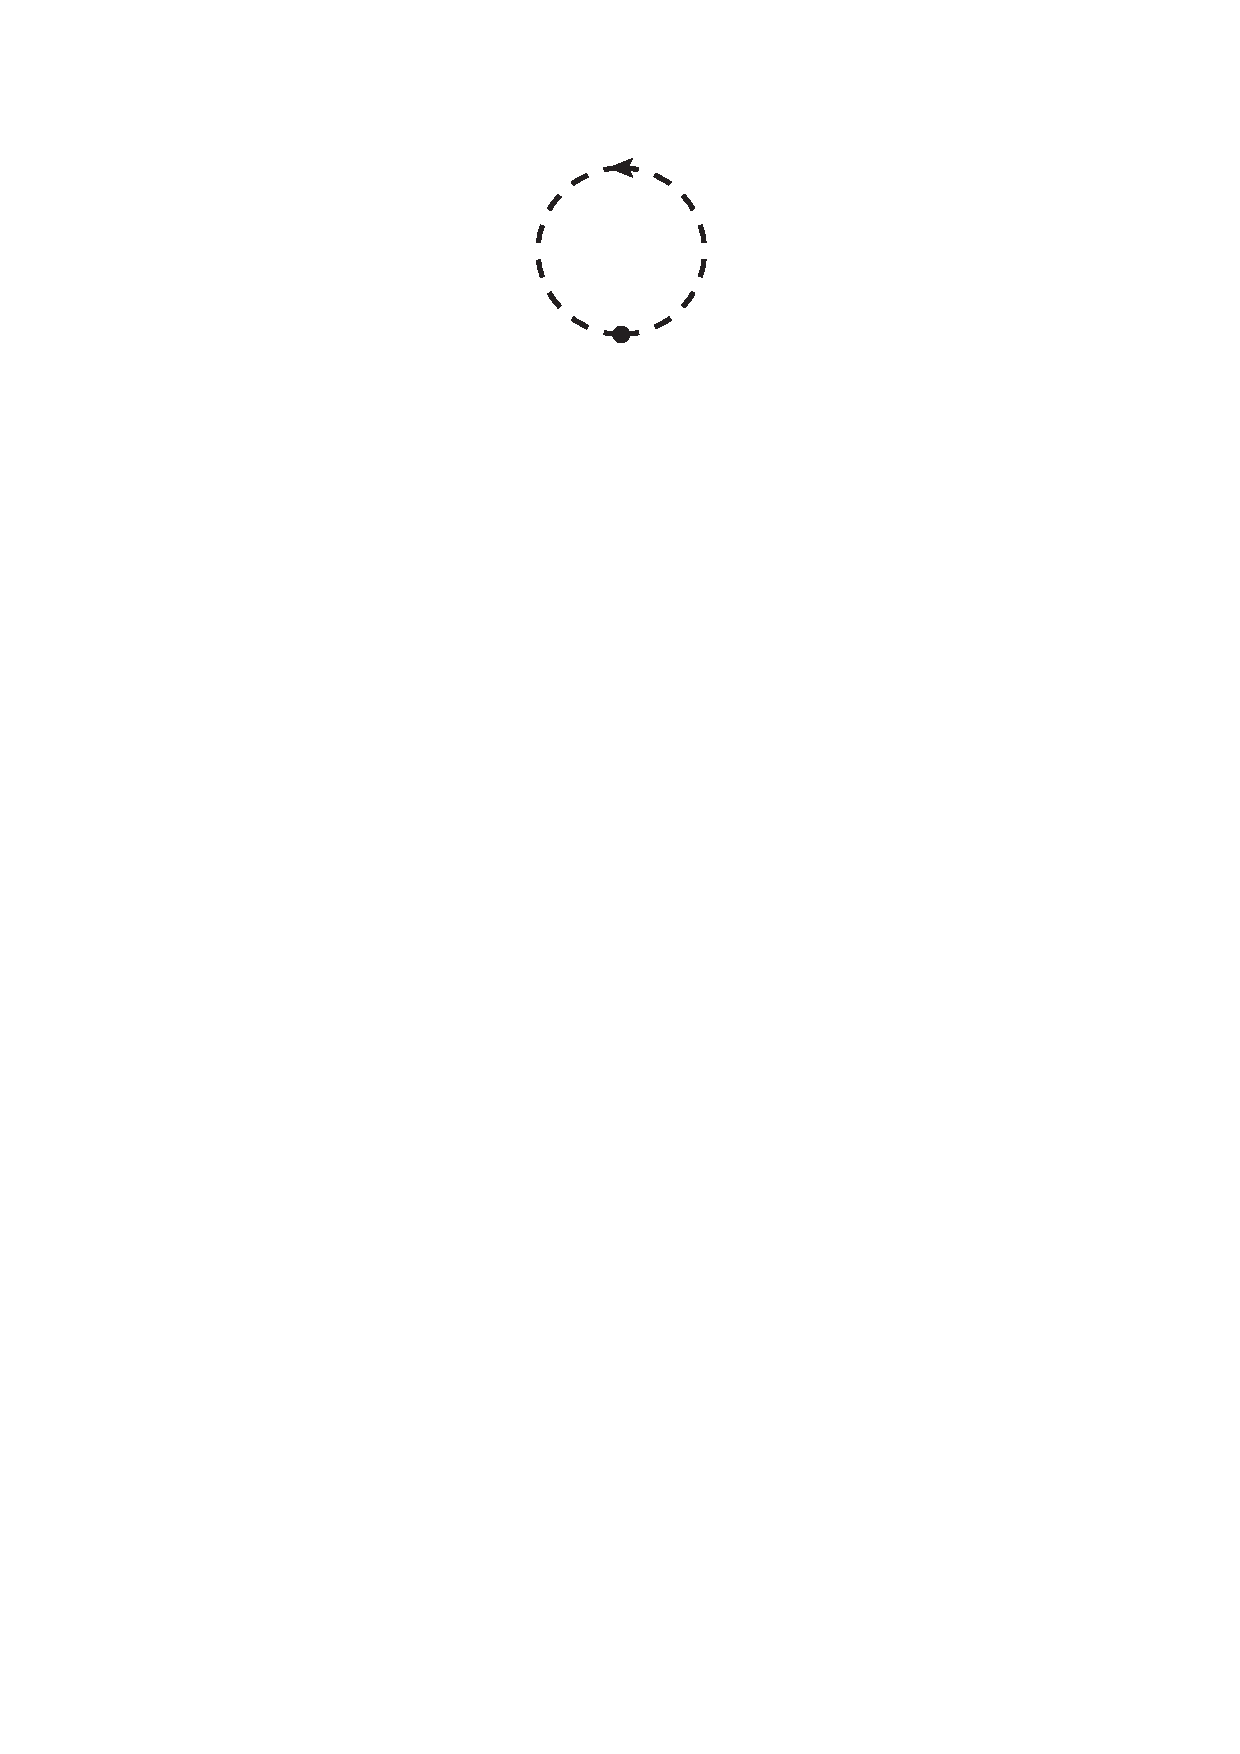
\includegraphics[trim={7cm 23cm 9cm 2cm}, clip=true,width=  2.5cm]{images/types of loops/meson.pdf}
\centering
\end{figure}

When a single meson make a loop, following type of integral appears

\beq
H = \int \tilde{d^dk} \frac{   {1}    }{  \left[k^2-M_\pi^2 \right] } 
\eeq   

\subsubsection{I integral}

\begin{figure}[h]
	\caption{Meson and baryon loop}
	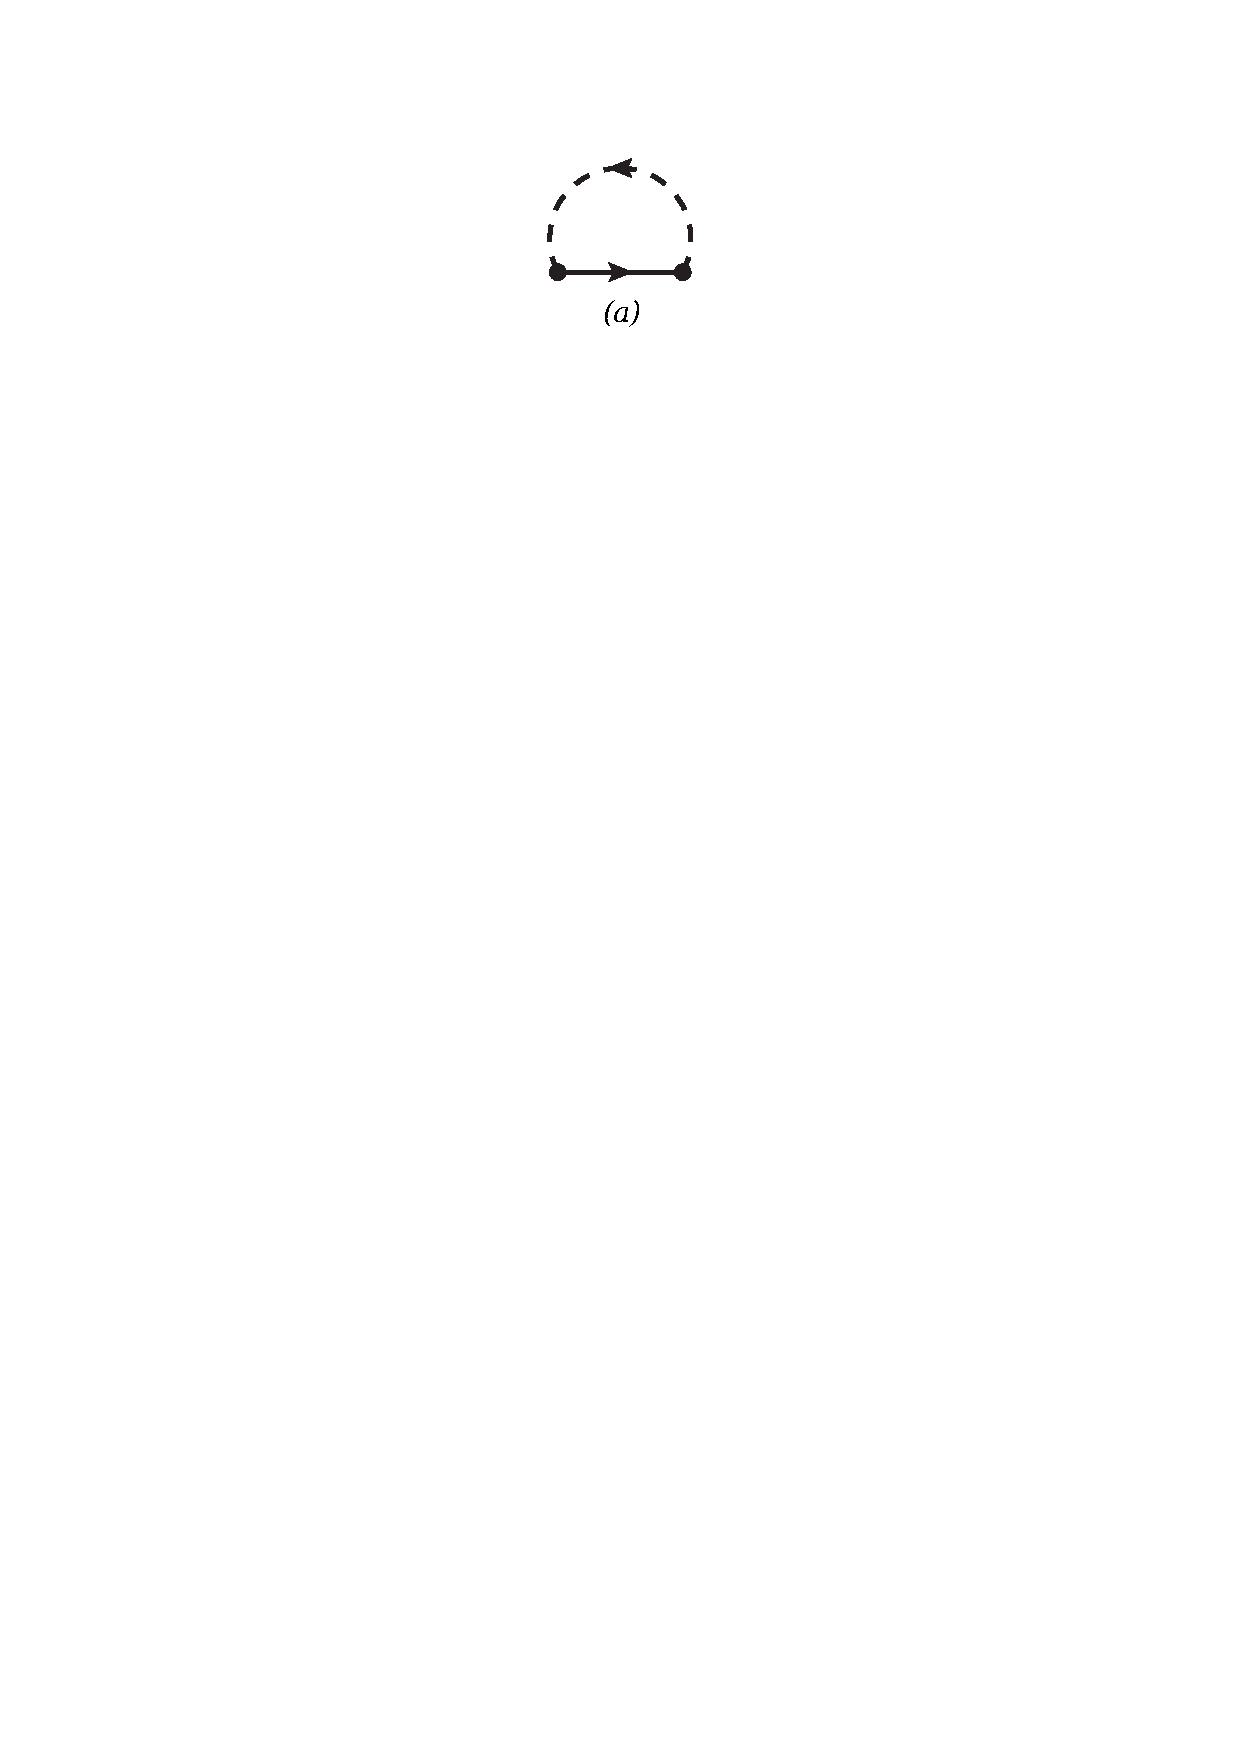
\includegraphics[trim={7cm 24cm 7cm 2cm}, clip=true,width=  3cm]{images/types of loops/meson_baryon_e.pdf}
	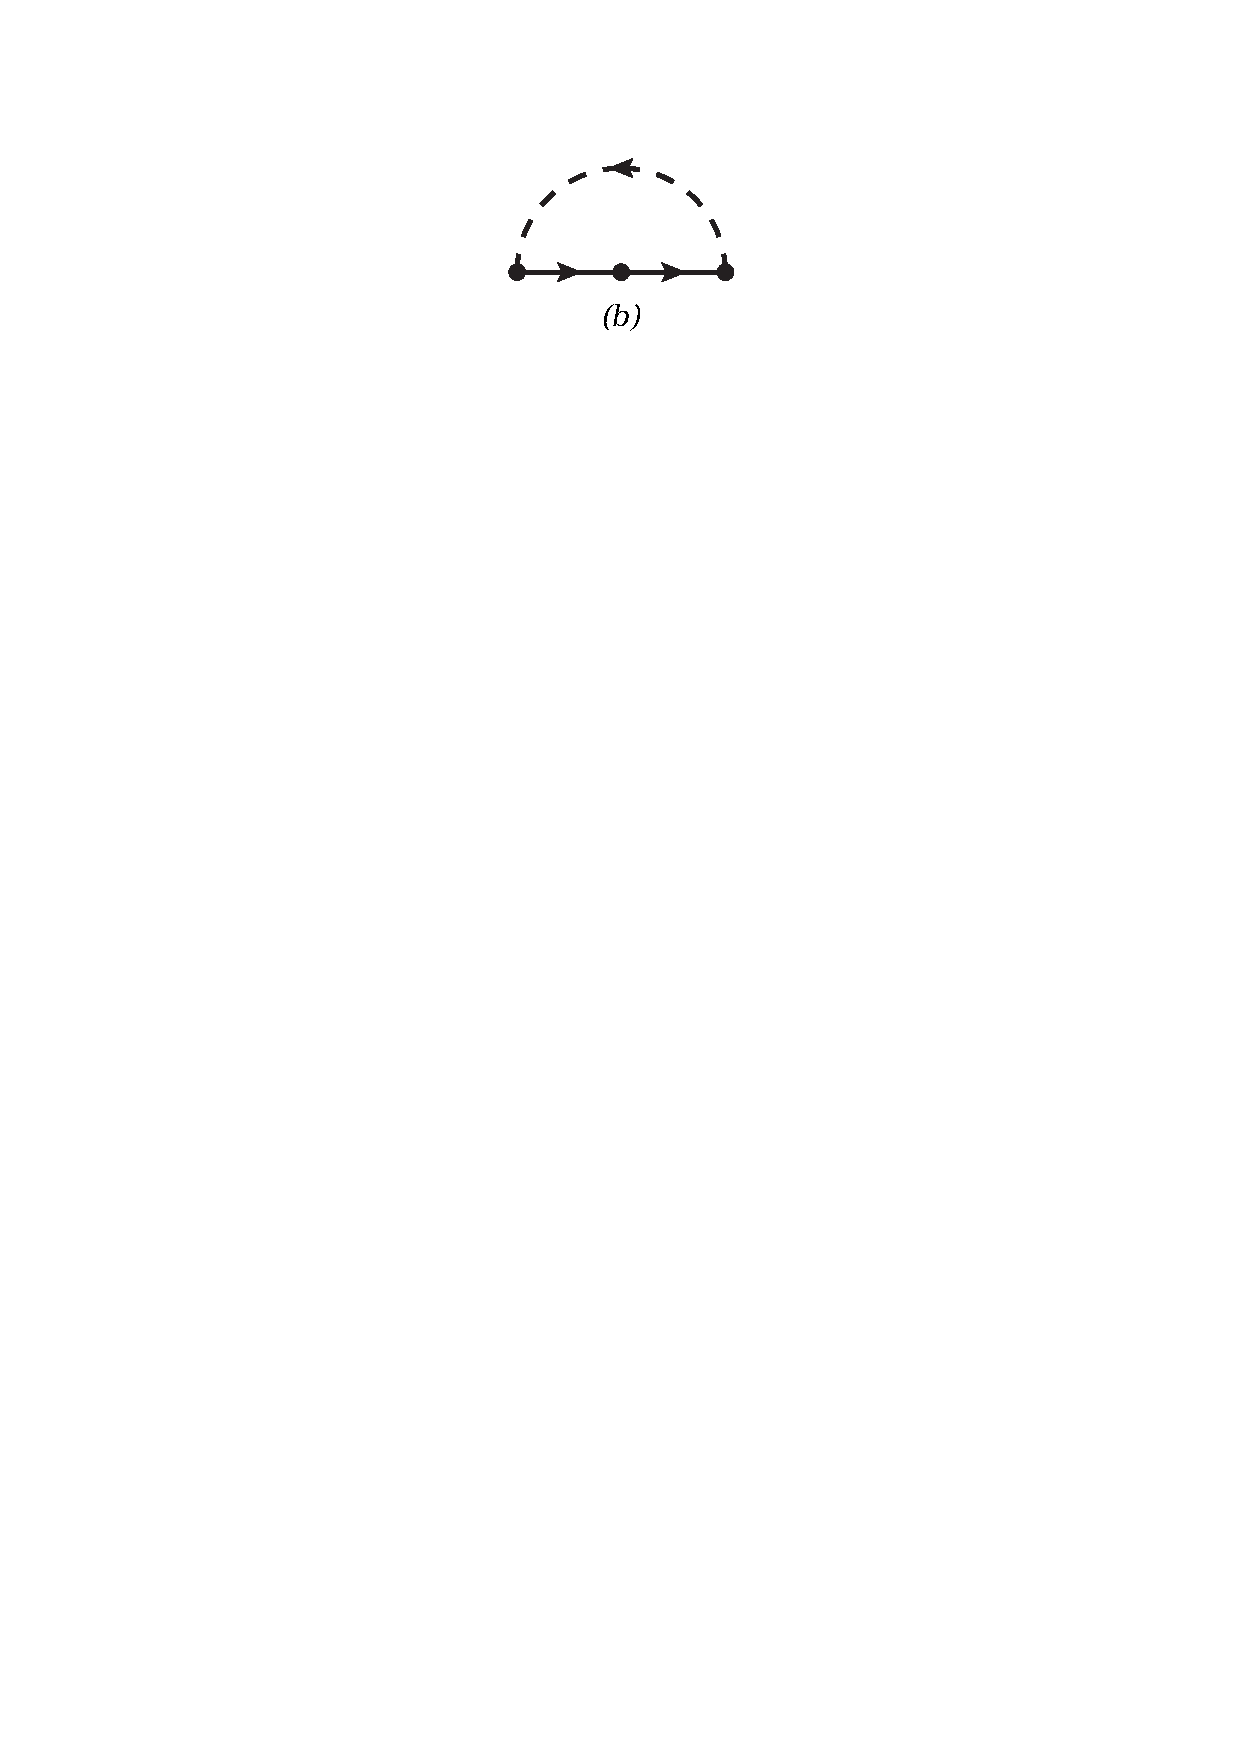
\includegraphics[trim={7cm 24cm 7cm 2cm}, clip=true,width=  3cm]{images/types of loops/meson_2baryon_e.pdf}
	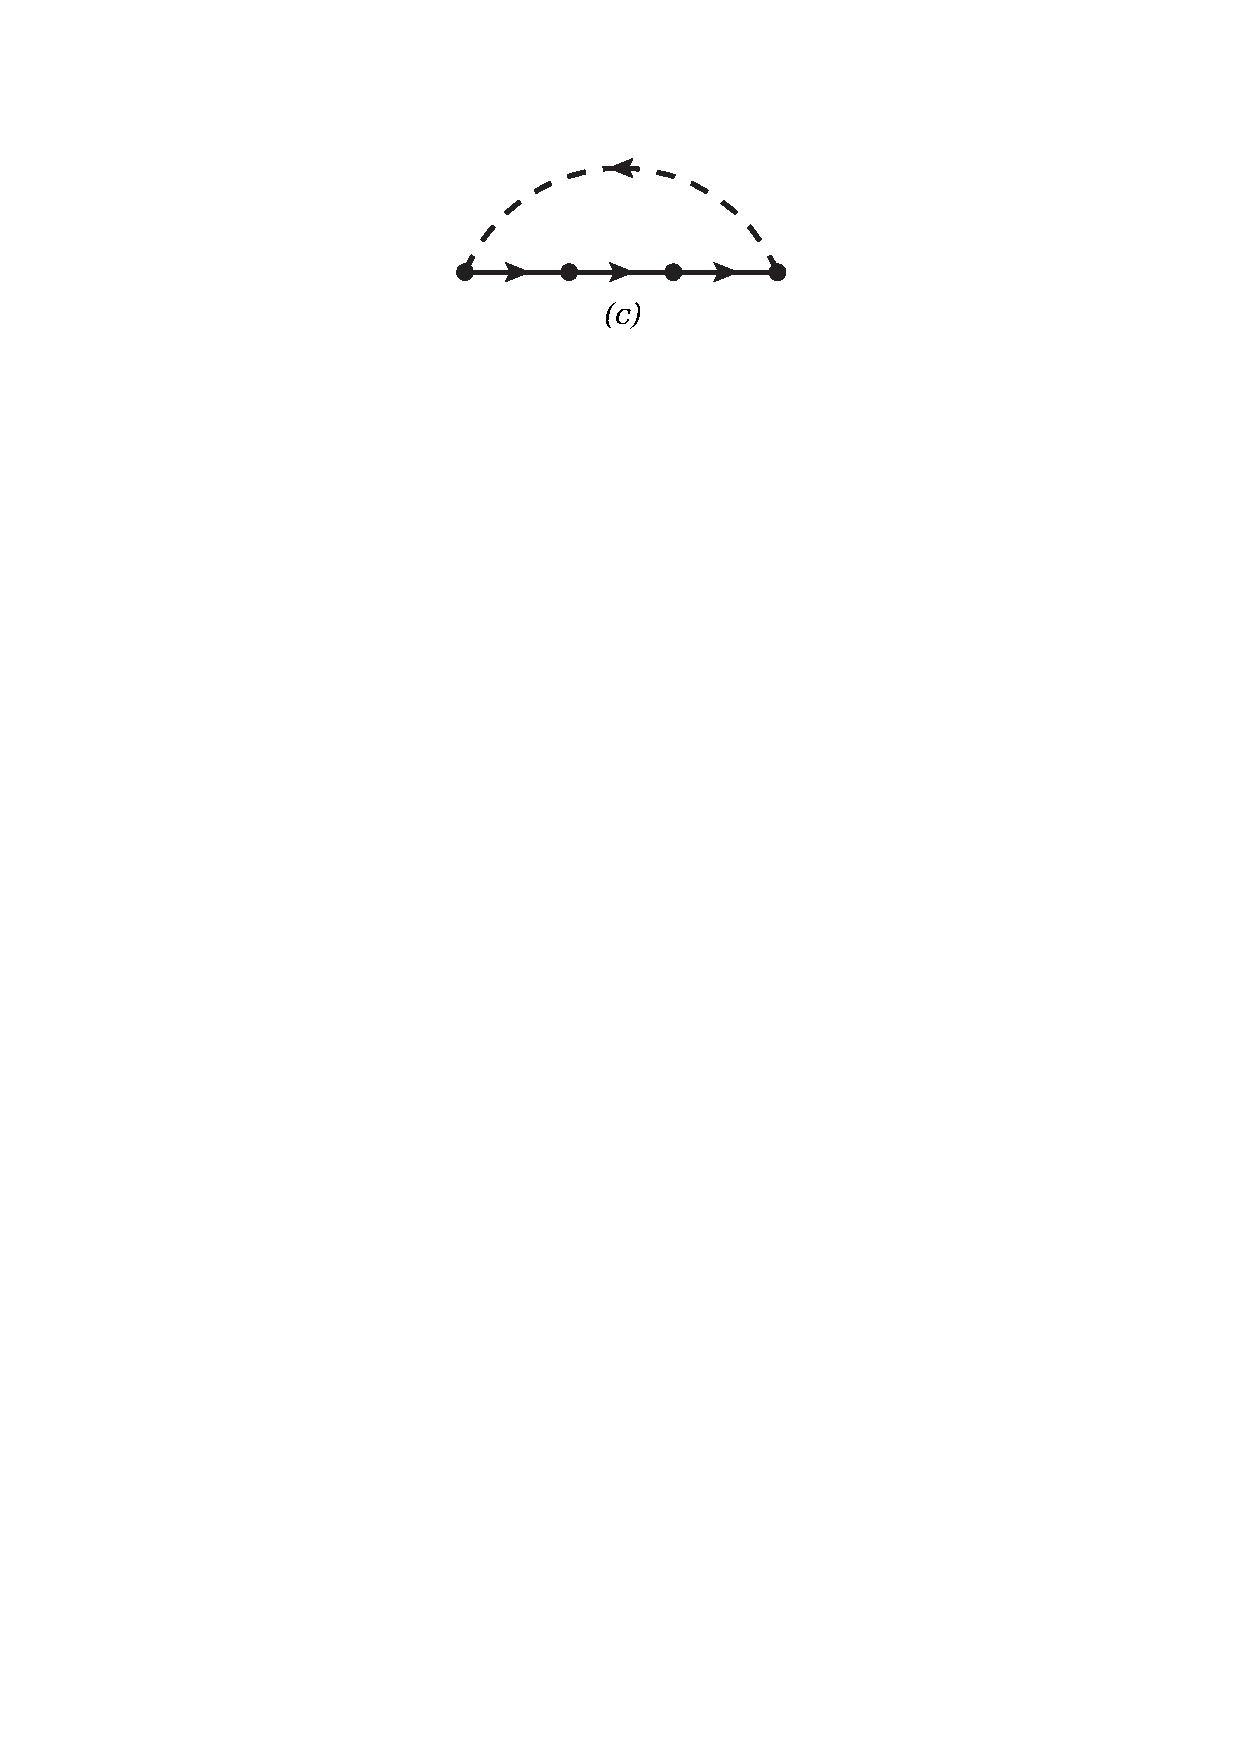
\includegraphics[trim={7cm 24cm 7cm 2cm}, clip=true,width=  3cm]{images/types of loops/meson_3baryon_e.pdf}
	\centering
\end{figure}

When a single meson and a single baryon make a loop (a), following type of integral appears

\beq
I = \int \tilde{d^dk} \frac{   {1}    }{ \left[ \left(p-k\right)^0 -\delta m_n \right] \left[k^2-M_\pi^2 \right] } 
\eeq   

Loop integrals with two or more baryons and a meson (b,c) can also be simplified to above type by decomposing baryon propagators into partial fractions.

\subsubsection{J integral}

\begin{figure}[h]
	\caption{Two meson loop}
	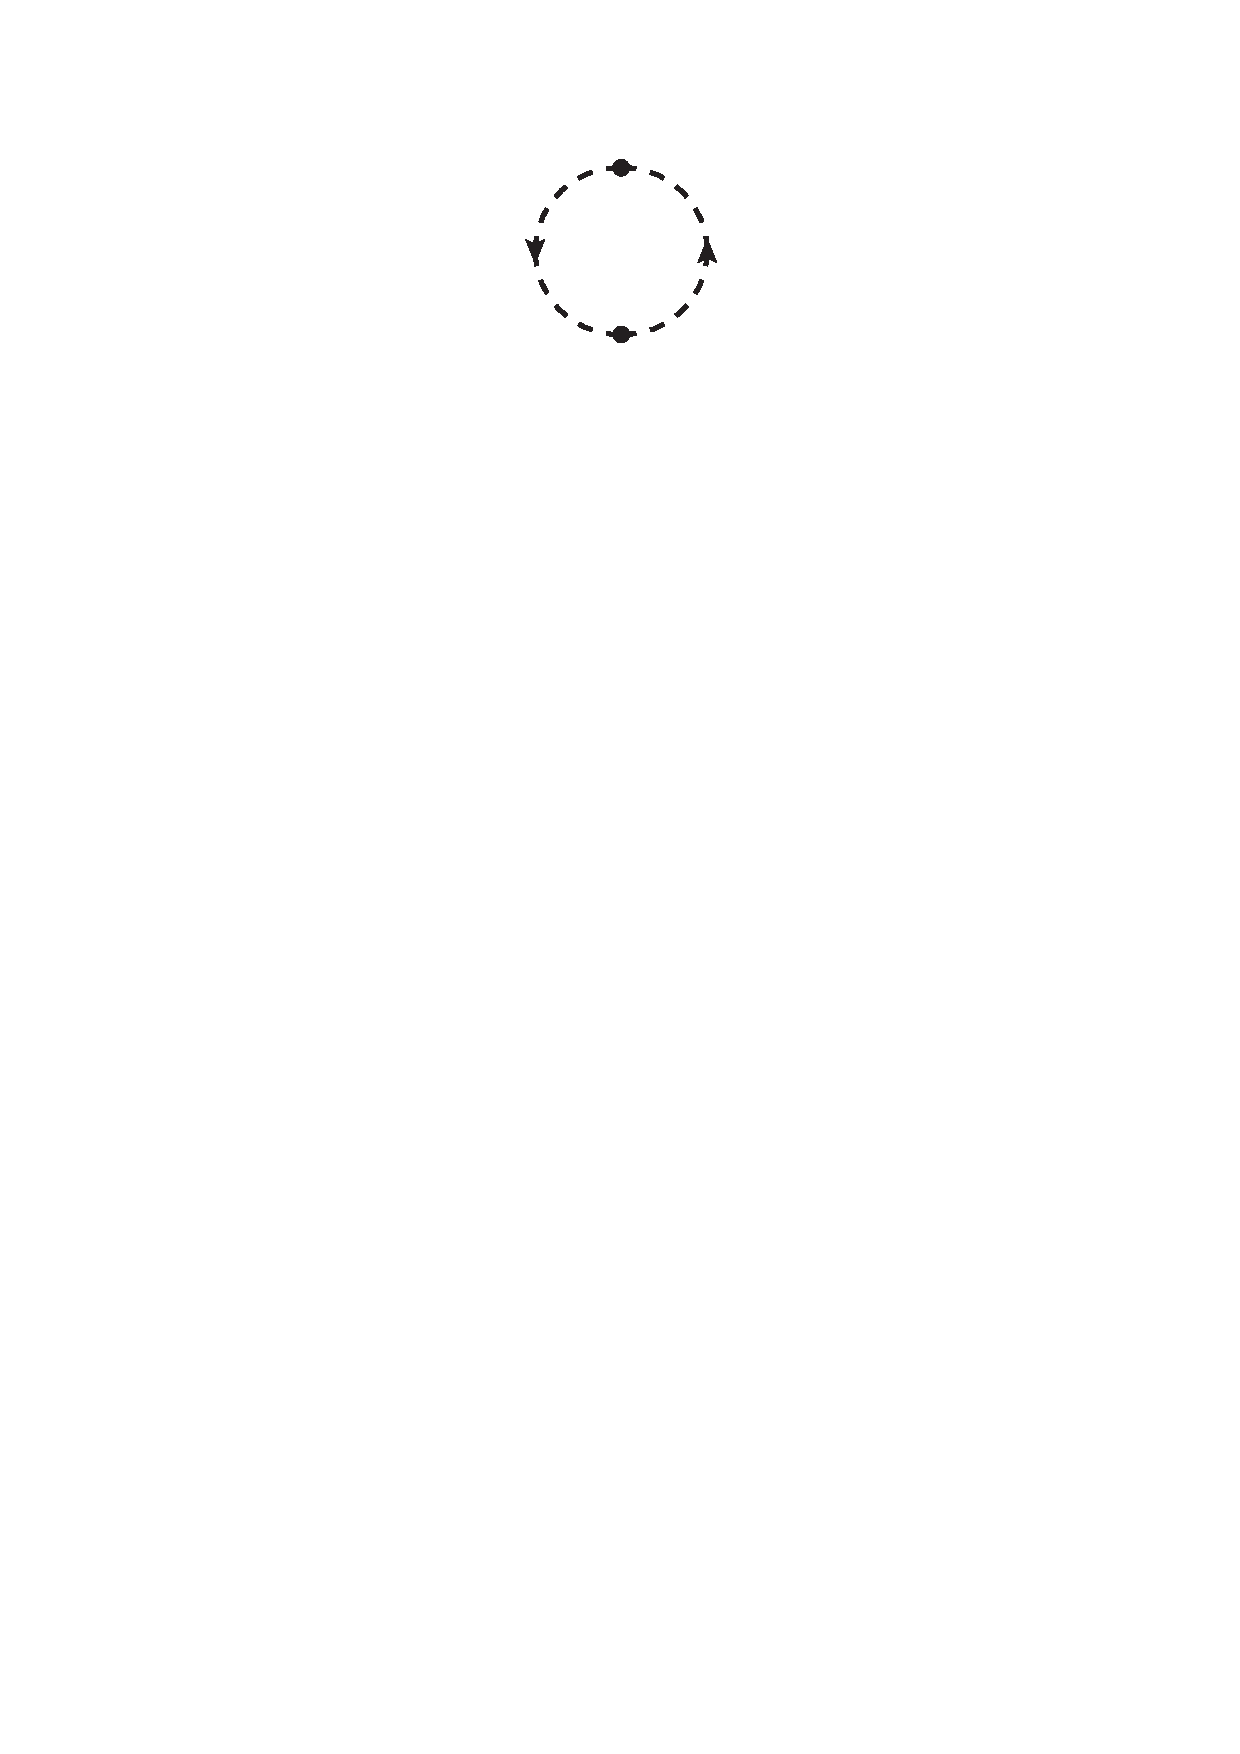
\includegraphics[trim={8cm 23.5cm 8cm 2cm}, clip=true,width=  2.5cm]{images/types of loops/2meson.pdf}
	\centering
\end{figure}

When two mesons make a loop, following type of integral appears

\beq
H = \int \tilde{d^dk} \frac{   {1}    }{ \left[k^2-M_\pi^2 \right] \left[(k+q)^2-M_\pi^2 \right] } 
\eeq   


\subsubsection{J$\Delta$ integral}

\begin{figure}[h]
	\caption{Baryon and two meson loop}
	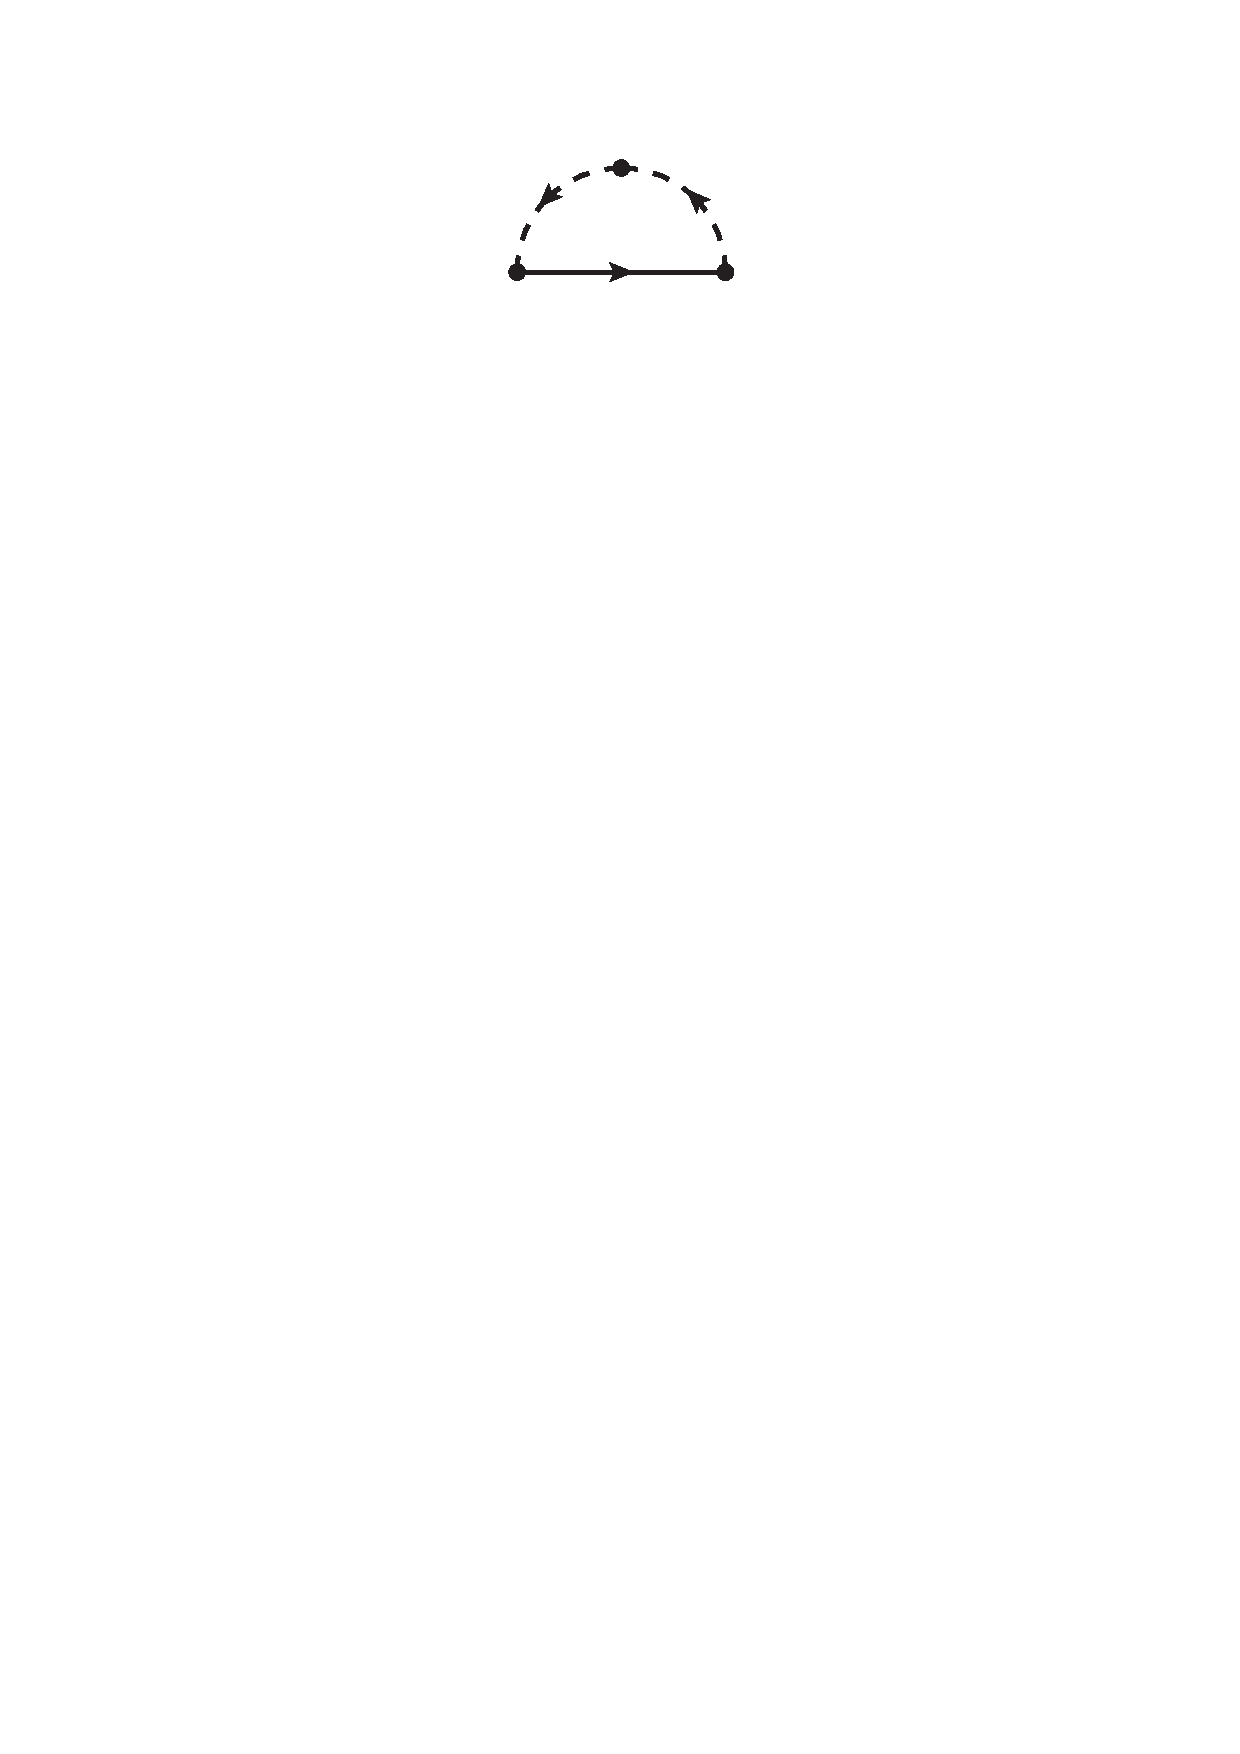
\includegraphics[trim={8cm 23.5cm 8cm 2cm}, clip=true,width=  2.5cm]{images/types of loops/2meson_baryon.pdf}
	\centering
\end{figure}

When a baryon and two mesons make a loop, following type of integral appears

\beq
H = \int \tilde{d^dk} \frac{   {1}    }{ \left[ \left(p-k\right)^0 -\delta m_n \right] \left[k^2-M_\pi^2 \right] \left[(k+q)^2-M_\pi^2 \right] } 
\eeq   



\subsection{Evaluating Loop Integrals}

\vspace{1mm}
Following steps were used to evaluate loop integrals.

\begin{enumerate}
	\item Feynman parameter integrals
	\beq
	\frac{1}{AB} =  \int_{0}^{\infty}   \frac{d\lambda}{ \left[ A+\lambda B \right] ^2 } \nonumber
	\eeq
	\item Wick rotation to convert Minkowski vector into a Euclidian vector
	\item Standard integral for Euclidian vectors \cite{Ramond}
	\beq
	\int \frac{d^dk}{ \left[ k^2+\Lambda^2 \right] ^n } =  \pi^{d/2}  \frac{ \Gamma \left( n-d/2 \right) }{\Gamma \left( n \right)} \frac{1}{ \left[ \Lambda^2 \right] ^{(n-d/2)} } \nonumber
	\eeq
\end{enumerate}


\bea
\int \tilde{d^dk} \frac{   \{ 1 ; k^0 ; k^i ; k^0k^i ; (k^0)^2 ; k^ik^j  \}    }{ \left[ \left(p-k\right)^0 -\delta m_n \right] \left[k^2-M_\pi^2 \right] } 
=\frac{2i}{ \left( 4\pi \right)^{d/2} }  \int_{0}^{\infty}d\lambda      \{ \Gamma \left( 2-d/2 \right) \left[ \Lambda^2 \right]^{(d/2-2)}&&;
\nonumber  \\
\Gamma \left( 2-d/2 \right)\lambda\left[ \Lambda^2 \right]^{(d/2-2)}&&;
\nonumber  \\
0  && ;
\nonumber  \\
0  &&;
\nonumber  \\
\Gamma \left( 2-d/2 \right)\lambda^2 \left[ \Lambda^2 \right]^{(d/2-2)} - \frac{1}{2} \Gamma \left( 1-d/2 \right) \left[ \Lambda^2 \right]^{(d/2-1)} && ;
\nonumber  \\
\frac{\delta^{i,j}}{2} \Gamma \left(1-d/2 \right) \left[ \Lambda^2 \right]^{(d/2-1)} && \}
\nonumber
\eea


\newpage
\subsubsection{I integrals}

\bea
I \left( n,p^0,M_\pi \right) && \equiv  \int \tilde{d^dk} \frac{  1  }{ \left[ p^0 -k^0 -\delta m_n \right] \left[k^2-M_\pi^2 \right] }
\nonumber\\
&& =\frac{2i}{ \left( 4\pi \right)^{d/2} }  \int_{0}^{\infty}d\lambda      \Gamma \left( 2-d/2 \right) \left[ \Lambda^2 \right]^{(d/2-2)}
\nonumber\\
&& =\frac{2i}{ \left( 4\pi \right)^{d/2} }    \Gamma \left( 2-d/2 \right) J \left( 2,0 \right)
\nonumber\\	[10pt]	
I_{0} \left( n,p^0,M_\pi \right) && \equiv  \int \tilde{d^dk} \frac{  k^0  }{ \left[ p^0 -k^0 -\delta m_n \right] \left[k^2-M_\pi^2 \right] }
\nonumber\\
&& =\frac{2i}{ \left( 4\pi \right)^{d/2} }  \int_{0}^{\infty}d\lambda     \Gamma \left( 2-d/2 \right)\lambda\left[ \Lambda^2 \right]^{(d/2-2)}
\nonumber\\
&& =\frac{2i}{ \left( 4\pi \right)^{d/2} }    \Gamma \left( 2-d/2 \right)  \left[ J\left(2,1\right)+ \lambda_0 J\left(2,0\right) \right]
\nonumber\\	[10pt]
I_{i} \left( n,p^0,M_\pi \right) && \equiv  \int \tilde{d^dk} \frac{  k^i  }{ \left[ p^0 -k^0 -\delta m_n \right] \left[k^2-M_\pi^2 \right] }
\nonumber\\
&& =0
\nonumber\\ [10pt]
I_{0i} \left( n,p^0,M_\pi \right) && \equiv  \int \tilde{d^dk} \frac{ k^0 k^i  }{ \left[ p^0 -k^0 -\delta m_n \right] \left[k^2-M_\pi^2 \right] }
\nonumber\\
&& =0
\nonumber\\ [10pt]
I_{00} \left( n,p^0,M_\pi \right) && \equiv  \int \tilde{d^dk} \frac{ (k^0)^2  }{ \left[ p^0 -k^0 -\delta m_n \right] \left[k^2-M_\pi^2 \right] }
\nonumber\\
&& = \frac{2i}{ \left( 4\pi \right)^{d/2} }  \int_{0}^{\infty}d\lambda   \{\Gamma \left( 2-d/2 \right)\lambda^2 \left[ \Lambda^2 \right]^{(d/2-2)} - \frac{1}{2} \Gamma \left( 1-d/2 \right) \left[ \Lambda^2 \right]^{(d/2-1)} \}
\nonumber\\
&& =\frac{i}{ \left( 4\pi \right)^{d/2} }   \{ 2 \Gamma \left( 2-d/2 \right)  \left[ J\left(2,2\right)+  2\lambda_0 J\left(2,1\right)  +\lambda_0^2 J\left(2,0\right) \right] -\Gamma \left( 1-d/2 \right) J\left(1,0\right) \}
\nonumber\\	[10pt]
I_{ij} \left( n,p^0,M_\pi \right) && \equiv  \int \tilde{d^dk} \frac{ k^i k^j  }{ \left[ p^0 -k^0 -\delta m_n \right] \left[k^2-M_\pi^2 \right] }
\nonumber\\
&& = \frac{2i}{ \left( 4\pi \right)^{d/2} }  \int_{0}^{\infty}d\lambda  \frac{\delta^{i,j}}{2} \Gamma \left(1-d/2 \right) \left[ \Lambda^2 \right]^{(d/2-1)}
\nonumber \\
&& = \frac{i \delta^{i,j}}{ \left( 4\pi \right)^{d/2} }  \Gamma \left(1-d/2 \right) J\left(1,0\right)
\nonumber 
\eea


Here $ \int \tilde{d^dk} = \int \frac{d^dk}{\left( 2\pi \right)^d }$, $ \Lambda^2= \lambda^2 -2\lambda \left( p^0-\delta m_n \right) + M_\pi ^2$ ,$ c_0= M_\pi^2-\left( p^0-\delta m_n\right)^2 $, $c_1=1$, and $\lambda_0 =p^0-\delta m_n$




\subsubsection{J$\Delta$ integrals}


\bea
	J \Delta_{1} \left(p,q,M  \right)=  && \equiv  \int \tilde{d^dk} \frac{   1    }{ \left[ \left(p-k\right)^0 \right] \left[\left( k+q \right) ^2-M^2 \right]  \left[k^2-M^2 \right] } 
	\nonumber\\
	&& =\frac{-2i  }{\left( 4\pi \right)^{d/2}} \Gamma \left(  3- d/2 \right)\int_{0}^{\infty}d \lambda \int_{0}^{1}d \alpha \left( \frac{1}{\Lambda} \right)^{3-d/2}
	\nonumber
	\nonumber\\	[10pt]
	J \Delta _{ k_\mu} \left(p,q,M  \right)=  && \equiv  \int \tilde{d^dk} \frac{   k_\mu    }{ \left[ \left(p-k\right)^0 \right] \left[\left( k+q \right) ^2-M^2 \right]  \left[k^2-M^2 \right] } 
	\nonumber\\
	&& =\frac{-2i  }{\left( 4\pi \right)^{d/2}} \Gamma \left(  3- d/2 \right)\int_{0}^{\infty}d \lambda \int_{0}^{1}d \alpha \left( \frac{1}{\Lambda} \right)^{3-d/2} \delta k_\mu
	\nonumber
	\nonumber\\	[10pt]
	J \Delta _{ k_\mu k_\nu } \left(p,q,M  \right)=  && \equiv  \int \tilde{d^dk} \frac{   k_\mu k_\nu   }{ \left[ \left(p-k\right)^0 \right] \left[\left( k+q \right) ^2-M^2 \right]  \left[k^2-M^2 \right] } 
	\nonumber\\
	&& =\frac{2i}{\left( 4\pi \right)^{d/2}}  \Gamma \left(  2- d/2 \right) \int_{0}^{\infty}d \lambda \int_{0}^{1}d \alpha \left( \frac{1}{\Lambda} \right)^{2-d/2} \left(  \frac{g_{\mu \nu}}{2} -\frac{\left(2-d/2\right)}{\Lambda}\delta k_\mu \delta k_\nu \right) 
	\nonumber\\
	J \Delta _{ k_\mu k_\nu k_\sigma} \left(p,q,M  \right)=  && \equiv  \int \tilde{d^dk} \frac{   k_\mu k_\nu  k_\sigma }{ \left[ \left(p-k\right)^0 \right] \left[\left( k+q \right) ^2-M^2 \right]  \left[k^2-M^2 \right] } 
	\nonumber\\
	&& =\frac{2i }{\left( 4\pi \right)^{d/2}}  \Gamma \left(  2- d/2 \right)\int_{0}^{\infty}d \lambda \int_{0}^{1}d \alpha \left( \frac{1}{\Lambda} \right)^{2-d/2} 
	\nonumber\\
	&& \qquad \qquad \qquad \qquad \left(  \frac{\delta k_\mu g_{\nu \sigma}+\delta k_\nu g_{\mu \sigma}+\delta k_\sigma g_{\mu \nu}}{2} -
	\frac{\left(2-d/2\right)}{\Lambda}\delta k_\mu \delta k_\nu \delta k_\sigma \right) 
	\nonumber
	\nonumber\	
\eea




\newpage
\begin{center}
		\begin{tabular}{ | m{5em} | m{12cm}|  } 
		\hline
		
		Integrals		
		& Results after the d-dimensional integral \\
		
		\hline
		$ J \Delta_{1} $
		
		&	\bea \frac{-2i  }{\left( 4\pi \right)^{d/2}}\int_{0}^{\infty}d \lambda \int_{0}^{1}d  \alpha\quad  \Gamma \left(  3- d/2 \right) \left( \frac{1}{\Lambda} \right)^{3-d/2} \nonumber \eea
		
		\\
		\hline
		$J \Delta _{ k_\mu} $
		
		& 	\bea\frac{-2i  }{\left( 4\pi \right)^{d/2}} \int_{0}^{\infty}d \lambda \int_{0}^{1}d \alpha \quad \Gamma \left(  3- d/2 \right)\left( \frac{1}{\Lambda} \right)^{3-d/2} \delta k_\mu
		\nonumber \eea 
		
		\\
		\hline
		$J \Delta _{  k_\mu k_\nu} $
		
		& \bea \frac{-2i}{\left( 4\pi \right)^{d/2}}  \int_{0}^{\infty}d \lambda \int_{0}^{1}d \alpha \bigg(  -\Gamma \left(  2- d/2 \right)\left( \frac{1}{\Lambda} \right)^{2-d/2} \frac{g_{\mu \nu}}{2} \nonumber\\  
		+ \Gamma \left(  3- d/2 \right)\left( \frac{1}{\Lambda} \right)^{3-d/2} \delta k_\mu \delta k_\nu \bigg) \nonumber \eea
		
		\\
		\hline
		$J \Delta _{  k_\mu k_\nu k_\rho} $
		
		& \bea \frac{-2i }{\left( 4\pi \right)^{d/2}}  \int_{0}^{\infty}d \lambda \int_{0}^{1}d \alpha 
		  \bigg(-\Gamma \left(  2- d/2 \right)\left( \frac{1}{\Lambda} \right)^{2-d/2}  \frac{1}{2}\left( \delta k_\mu g_{\nu \rho}+\delta k_\nu g_{\mu \rho}+\delta k_\rho g_{\mu \nu}\right)\nonumber\\ + \Gamma \left(  3- d/2 \right)\left( \frac{1}{\Lambda} \right)^{3-d/2}
		\delta k_\mu \delta k_\nu \delta k_\rho \bigg) \nonumber \eea
		
		\\
		\hline
		$J \Delta _{  k_\mu k_\nu k_\rho k_\sigma} $
		
		& \bea \frac{-2i }{\left( 4\pi \right)^{d/2}}  \int_{0}^{\infty}d \lambda \int_{0}^{1}d \alpha 
		\bigg(\Gamma \left(  1- d/2 \right)\left( \frac{1}{\Lambda} \right)^{1-d/2}  \frac{1}{4}\left( g_{\mu \nu} g_{\rho \sigma}+g_{\mu \rho} g_{\nu \sigma}+g_{\mu \sigma} g_{\nu \rho} \right)\nonumber\\ + \Gamma \left(  3- d/2 \right)\left( \frac{1}{\Lambda} \right)^{3-d/2}
		\delta k_\mu \delta k_\nu \delta k_\rho \delta k_\sigma  \nonumber\\
		-\Gamma \left(  2- d/2 \right)\left( \frac{1}{\Lambda} \right)^{2-d/2}  \frac{1}{2}\big( g_{\mu \nu} \delta k_\rho \delta k_\sigma +g_{\mu \rho} \delta k_\nu \delta k_\sigma +g_{\mu \sigma} \delta k_\rho \delta k_\nu\nonumber\\+g_{\nu \rho} \delta k_\mu \delta k_\sigma+g_{\sigma \nu} \delta k_\rho \delta k_\mu+g_{\rho \sigma} \delta k_\mu \delta k_\nu \big) \bigg) \nonumber \eea
		
		\\
		\hline
	\end{tabular}
	\end{center}
 
	\bea
	\Lambda^2 =  \left( \lambda- \lambda_0\right)^2 + c_0\nonumber\\
	c_0 = M^2-\lambda_0^2 -\alpha \left( 1-\alpha\right)q^2 ;&&\quad \delta k_0 = \lambda-  \left( 1-\alpha\right)q_0\nonumber \\
		\lambda_0 = p_0 +  \left( 1-\alpha\right)q_0  ;&& \quad \delta k_i = -  \left( 1-\alpha\right)q_i  \nonumber
	\eea


\newpage
\begin{center}	
	\begin{tabular}{ | m{5em} | m{11.7cm}|  } 
		\hline
		
		Integrals		
		& Result \\
		
		\hline
		$ J \Delta_{1} $
		
		&	\bea \frac{-2i  }{\left( 4\pi \right)^{d/2}} \int_{0}^{1}d \alpha \quad \Gamma \left(  3- d/2 \right) J\left(3,0\right) \nonumber \eea
		
		\\
		\hline
		$J \Delta _{ k_i} $
		
		& 	\bea\frac{-2i  }{\left( 4\pi \right)^{d/2}} \int_{0}^{1}d \alpha \quad \Gamma \left(  3- d/2 \right)J(3,0) \delta k_i
		\nonumber \eea 
		
				\\
		\hline
		$J \Delta _{ k_0} $
		
		& 	\bea\frac{-2i  }{\left( 4\pi \right)^{d/2}} \int_{0}^{1}d \alpha \quad \Gamma \left(  3- d/2 \right)\left( J(3,1)+J(3,0) p_0 \right)
		\nonumber \eea 
		
		
		\\
		\hline
		$J \Delta _{  k_i k_j} $
		
		& \bea \frac{-2i}{\left( 4\pi \right)^{d/2}}  \int_{0}^{1}d \alpha \bigg(  -\Gamma \left(  2- d/2 \right) J(2,0) \frac{g_{i j}}{2}  
		+ \Gamma \left(  3- d/2 \right) J(3,0) \delta k_i \delta k_j \bigg) \nonumber \eea
		
		
		\\
		\hline
		$J \Delta _{  k_0 k_j} $
		
		& \bea \frac{-2i}{\left( 4\pi \right)^{d/2}}  \int_{0}^{1}d \alpha \quad \Gamma \left(  3- d/2 \right) \left( J(3,1) +J(3,0)p_0  \right) \delta k_j  \nonumber \eea
		
		\\
		\hline
		$J \Delta _{  k_0 k_0} $
		
		& \bea \frac{-2i}{\left( 4\pi \right)^{d/2}}  \int_{0}^{1}d \alpha \bigg(  -\frac{1}{2} \Gamma \left(  2- d/2 \right) J(2,0)  \quad\quad\quad\quad\quad\quad \nonumber\\
		+ \Gamma \left(  3- d/2 \right) \left( J(3,2)+2J(3,1) p_0+ J(3,0)p_0^2 \right) \bigg) \nonumber \eea
				
		
		\\
		\hline
		$J \Delta _{  k_i k_j k_l} $
		
		& \bea \frac{-2i }{\left( 4\pi \right)^{d/2}} \int_{0}^{1}d \alpha 
		\bigg(-\frac{1}{2}\Gamma \left(  2- d/2 \right) J(2,0) \left( \delta k_i g_{j l}+\delta k_j g_{i l}+\delta k_l g_{i j}\right)\nonumber\\ + \Gamma \left(  3- d/2 \right)J(3,0)
		\delta k_i \delta k_j \delta k_l \bigg) \nonumber \eea
		
		
		
		\\
		\hline
		\end{tabular}
	\end{center}



\newpage
	\begin{center}	
		\begin{tabular}{ | m{5em} | m{11.7cm}|  } 
		\hline
		$J \Delta _{  k_0 k_j k_l} $
		
		& \bea \frac{-2i }{\left( 4\pi \right)^{d/2}} \int_{0}^{1}d \alpha 
		\bigg(-\frac{1}{2} \Gamma \left(  2- d/2 \right)  \left( J(2,1)+J(2,0)p_0 \right) g_{j l}\nonumber\\ + \Gamma \left(  3- d/2 \right) \left(J(3,1)+ J(3,0)p_0 \right)
		\bigg) \delta k_j \delta k_l \nonumber \eea
		
			
			
		\\	
		\hline
		$J \Delta _{  k_0 k_0 k_l} $
		
		& \bea \frac{-2i }{\left( 4\pi \right)^{d/2}} \int_{0}^{1}d \alpha 
		\bigg(-\frac{1}{2} \Gamma \left(  2- d/2 \right) J(2,0) \delta k_l \quad\quad\quad\quad \nonumber\\ + \Gamma \left(  3- d/2 \right)\left( J(3,2)+2J(3,1) p_0+ J(3,0)p_0^2 \right) \delta k_l \bigg) \nonumber \eea
		
		\\
		\hline
		$J \Delta _{  k_0 k_0 k_0} $
		
		& \bea \frac{-2i }{\left( 4\pi \right)^{d/2}} \int_{0}^{1}d \alpha 
		\bigg(- \frac{3}{2} \Gamma \left(  2- d/2 \right) \left( J(2,1) +J(2,0)p_0 \right)\nonumber\\ + \Gamma \left(  3- d/2 \right) \left( J(3,3) +3J(3,2)p_0+ 3J(3,1)p_0^2+J(3,0)p_0^3 \right)
		\bigg) \nonumber \eea
			
		
		\\
		\hline
		$J \Delta _{  k_i k_j k_l k_m} $
		
		& \bea \frac{-2i }{\left( 4\pi \right)^{d/2}} \int_{0}^{1}d \alpha 
		\bigg(\frac{1}{4}\Gamma \left(  1- d/2 \right) J(1,0)  \left( g_{i j} g_{l m}+g_{i l} g_{j m}+g_{i m} g_{j l} \right)\nonumber\\ + \Gamma \left(  3- d/2 \right) J(3,0)
		\delta k_i \delta k_j \delta k_l \delta k_m  \nonumber\\
		-\frac{1}{2}\Gamma \left(  2- d/2 \right) J(2,0)\big( g_{i j} \delta k_l \delta k_m +g_{i l} \delta k_j \delta k_m +g_{i m} \delta k_l \delta k_j\nonumber\\+g_{j l} \delta k_i \delta k_m+g_{m j} \delta k_l \delta k_i+g_{l m} \delta k_i \delta k_j \big) \bigg) \nonumber \eea
		
		\\
		\hline
		$J \Delta _{  k_0 k_j k_l k_m} $
		
		& \bea \frac{-2i }{\left( 4\pi \right)^{d/2}} \int_{0}^{1}d \alpha 
		\bigg( \Gamma \left(  3- d/2 \right)  \left(J(3,1)+ J(3,0)p_0 \right) \delta k_j \delta k_l \delta k_m  \nonumber\\
		-\frac{1}{2}\Gamma \left(  2- d/2 \right)   \left(J(2,1)+ J(2,0)p_0 \right)\big( g_{j l} \delta k_m+g_{m j} \delta k_l +g_{l m}  \delta k_j \big) \bigg) \nonumber \eea
		
				
		\\
		\hline

		\end{tabular}
	\end{center}



\newpage
	\begin{center}	
		\begin{tabular}{ | m{5em} | m{11.7cm}|  } 
		\hline
		$J \Delta _{  k_0 k_0 k_l k_m} $
		
		& \bea \frac{-2i }{\left( 4\pi \right)^{d/2}} \int_{0}^{1}d \alpha 
		\bigg(\frac{1}{4} \Gamma \left(  1- d/2 \right) J(1,0)  g_{l m} \quad\quad\quad\quad\quad\quad\quad\quad \nonumber\\ + \Gamma \left(  3- d/2 \right) \left( J(3,2)+2J(3,1) p_0+ J(3,0)p_0^2 \right) \delta k_l \delta k_m  \nonumber\\
		-\frac{1}{2} \Gamma \left(  2- d/2 \right) \big(J(2,0) \delta k_l \delta k_m +  \left( J(2,2)+2J(2,1) p_0+ J(2,0)p_0^2 \right)g_{l m} \big) \bigg) \nonumber \eea
		
		\\
		\hline
		$J \Delta _{  k_0 k_0 k_0 k_m} $
		
		& \bea \frac{-2i }{\left( 4\pi \right)^{d/2}} \int_{0}^{1}d \alpha 
		\bigg( \Gamma \left(  3- d/2 \right) \left( J(3,3) +3J(3,2)p_0+ 3J(3,1)p_0^2+J(3,0)p_0^3 \right) \delta k_m  \nonumber\\
		-\frac{3}{2}\Gamma \left(  2- d/2 \right)\left( J(2,1)+J(2,0)p_0 \right) \delta k_m \bigg) \nonumber \eea
		

		\\
		\hline
		$J \Delta _{  k_0 k_0 k_0 k_0} $
		
		& \bea \frac{-2i }{\left( 4\pi \right)^{d/2}} \int_{0}^{1}d \alpha 
		\bigg(\frac{3}{4} \Gamma \left(  1- d/2 \right) J(1,0) \quad\quad\quad\quad\quad\quad\quad\quad\quad \nonumber\\ + \Gamma \left(  3- d/2 \right) \left( J(3,4)+4J(3,3)p_0+6J(3,2)p_0^2+4J(3,1)p_0^3+J(3,0)p_0^4 \right) \nonumber\\
		-3\Gamma \left(  2- d/2 \right)\left( J(2,2)+2J(2,1) p_0+ J(2,0)p_0^2 \right) \bigg) \nonumber \eea
		
		
		\\
		\hline
		
		\end{tabular}
	\end{center}

Where $ \delta k_i = -  \left( 1-\alpha\right)q_i $
\bea
J\left( \nu, n \right) = \int_{0}^{\infty} \left( \lambda-\lambda_0\right)^n \left[ c_0 + c_1 \left( \lambda-\lambda_0\right)^2   \right]^{d/2-\nu} d\lambda \nonumber
\eea




\newpage
\begin{center}	
	\begin{tabular}{ | m{5em} | m{12cm}|  } 
		\hline
		
		Integrals		
		& $1/\epsilon$ terms  \\
		
		\hline
		$ J \Delta_{1} $
		
		&	\bea 0 \nonumber \eea
		
		\\
		\hline
		$J \Delta _{ k_i} $
		
		& 	\bea 0 
		\nonumber \eea 
		
		\\
		\hline
		$J \Delta _{ k_0} $
		
		& 	\bea -\frac{i}{16 \pi^2}  
		\nonumber \eea 
		
		
		
		\\
		\hline
		$J \Delta _{  k_i k_j} $
		
		& \bea -\frac{i}{32 \pi^2} \left( 2p_0+q_0\right) \delta_{ij} \nonumber \eea
		
		
		\\
		\hline
		$J \Delta _{  k_0 k_j} $
		
		& \bea \frac{i}{32 \pi^2} q_j \nonumber \eea
		
		
		\\
		\hline
		$J \Delta _{  k_0 k_0} $
		
		& \bea -\frac{i}{32 \pi^2} (2p_0-q_0) \nonumber \eea
		
		
		\\
		\hline
		$J \Delta _{  k_i k_j k_l} $
		
		& \bea \frac{i}{96 \pi^2} \left( 3p_0+2q_0\right) \left(q_i\delta_{jl}+ q_j\delta_{il} +q_l\delta_{ij} \right)\nonumber \eea
		
		\\
		\hline
		$J \Delta _{  k_0 k_j k_l} $
		
		& \bea -\frac{i}{192 \pi^2} \left( 4q_j q_l +(q^2+6p_0q_0+12p_0^2-6M^2) \delta_{jl}\right) \nonumber \eea
		
		\\
		\hline
		$J \Delta _{  k_0 k_0 k_l} $
		
		& \bea \frac{i}{96 \pi^2} \left( 3p_0-2q_0\right)q_l \nonumber \eea
		
		\\
		\hline
		$J \Delta _{  k_0 k_0 k_0} $
		
		& \bea -\frac{i}{192 \pi^2} \left( 6 M^2 + 12 p_0^2 - q^2 - 6 p_0 q_0 + 4 q_0^2 \right) \nonumber \eea
		
		\\
		\hline
	\end{tabular}
\end{center}


\newpage
\begin{center}	
	\begin{tabular}{ | m{5em} | m{12cm}|  } 
		\hline
		
		Integrals		
		& $1/\epsilon$ terms\\
		
		\hline
		$J \Delta _{  k_i k_j k_l k_m} $
		
		& \bea -\frac{i}{384 \pi^2} \bigg(\left( 2p_0+q_0\right) \left( q^2+4 p_0 q_0+4p_0^2+2q_0^2-6M^2\right) \left(\delta_{ij}\delta_{lm}+\delta_{il}\delta_{jm}+\delta_{im}\delta_{jl}\right)\nonumber\\ 
		+2 \left( 4p_0+3q_0\right)  \left(\delta_{ij} q_l q_m+\delta_{il}q_j q_m+\delta_{im}q_j q_l+ \delta_{jl}q_i q_m+\delta_{jm}q_iq_l+\delta_{lm}q_iq_j\right) \bigg)\nonumber \eea
		
		\\
		\hline
		$J \Delta _{  k_0 k_j k_l k_m} $
		
		& \bea -\frac{i}{384 \pi^2} \bigg((6 M^2 - 12 p_0^2 - q^2 - 8 p_0 q_0)(q_j \delta_{lm}+ q_l \delta_{jm} +q_m \delta_{jl}  ) -6 q_j q_l q_m\bigg)\nonumber \eea
		
		\\
		\hline
		$J \Delta _{  k_0 k_0 k_l k_m} $
		
		& \bea \frac{i}{384 \pi^2} \bigg( 2(3q_0-4p_0)q_lq_m +(6 M^2 (2 p_0 - q_0) - 12 p_0^2 q_0 + q^2 q_0 -24 p_0^3 - 2 p_0 q^2) \delta_{lm}\bigg)\nonumber \eea
		
		\\
		\hline
		$J \Delta _{  k_0 k_0 k_0 k_m} $
		
		& \bea \frac{i}{384 \pi^2} \bigg( 6 M^2 + 12 p_0^2 - q^2 - 8 p_0 q_0 + 6 q_0^2\bigg) q_m\nonumber \eea
		
		\\
		\hline
		$J \Delta _{  k_0 k_0 k_0 k_0} $
		
		& \bea - \frac{i}{384 \pi^2} \bigg( 24 p_0^3 - 2 p_0 q^2 + 6 M^2 (2 p_0 - 3 q_0) - 12 p_0^2 q_0 + 3 q^2 q_0 + 
		8 p_0 q_0^2 - 6 q_0^3\bigg) \nonumber \eea
		
		
		\\
		\hline
	\end{tabular}
\end{center}




\newpage
\begin{center}	
	\begin{tabular}{ | m{5em} | m{12cm}|  } 
		\hline
		
		Integrals		
		& Results when all indices are spatial \\
		
		\hline
		$ J \Delta_{1} $
		
		&	\bea \frac{-2i  }{\left( 4\pi \right)^{d/2}} \int_{0}^{1}d \alpha \quad \Gamma \left(  3- d/2 \right) J\left(3,0\right) \nonumber \eea
		
		\\
		\hline
		$J \Delta _{ k_i} $
		
		& 	\bea\frac{-2i  }{\left( 4\pi \right)^{d/2}} \int_{0}^{1}d \alpha \quad \Gamma \left(  3- d/2 \right)J(3,0) \delta k_i
		\nonumber \eea 
		
		\\
		\hline
		$J \Delta _{  k_i k_j} $
		
		& \bea \frac{-2i}{\left( 4\pi \right)^{d/2}}  \int_{0}^{1}d \alpha \bigg(  -\Gamma \left(  2- d/2 \right) J(2,0) \frac{g_{i j}}{2}  
		+ \Gamma \left(  3- d/2 \right) J(3,0) \delta k_i \delta k_j \bigg) \nonumber \eea
		
		\\
		\hline
		$J \Delta _{  k_i k_j k_l} $
		
		& \bea \frac{-2i }{\left( 4\pi \right)^{d/2}} \int_{0}^{1}d \alpha 
		\bigg(-\frac{1}{2}\Gamma \left(  2- d/2 \right) J(2,0) \left( \delta k_i g_{j l}+\delta k_j g_{i l}+\delta k_l g_{i j}\right)\nonumber\\ + \Gamma \left(  3- d/2 \right)J(3,0)
		\delta k_i \delta k_j \delta k_l \bigg) \nonumber \eea
		
		\\
		\hline
		$J \Delta _{  k_i k_j k_l k_m} $
		
		& \bea \frac{-2i }{\left( 4\pi \right)^{d/2}} \int_{0}^{1}d \alpha 
		\bigg(\frac{1}{4}\Gamma \left(  1- d/2 \right) J(1,0)  \left( g_{i j} g_{l m}+g_{i l} g_{j m}+g_{i m} g_{j l} \right)\nonumber\\ + \Gamma \left(  3- d/2 \right) J(3,0)
		\delta k_i \delta k_j \delta k_l \delta k_m  \nonumber\\
		-\frac{1}{2}\Gamma \left(  2- d/2 \right) J(2,0)\big( g_{i j} \delta k_l \delta k_m +g_{i l} \delta k_j \delta k_m +g_{i m} \delta k_l \delta k_j\nonumber\\+g_{j l} \delta k_i \delta k_m+g_{m j} \delta k_l \delta k_i+g_{l m} \delta k_i \delta k_j \big) \bigg) \nonumber \eea
		
		\\
		\hline
	\end{tabular}
\end{center}

Where $ \delta k_i = -  \left( 1-\alpha\right)q_i $
\bea
J\left( \nu, n \right) = \int_{0}^{\infty} \left( \lambda-\lambda_0\right)^n \left[ c_0 + c_1 \left( \lambda-\lambda_0\right)^2   \right]^{d/2-\nu} d\lambda \nonumber
\eea




\newpage
\begin{center}	
	\begin{tabular}{ | m{5em} | m{12cm}|  } 
		\hline
		
		Integrals		
		& Results when index $\mu = 0$ and all the other indices are spatial  \\
		
		\hline
		$ J \Delta_{1} $
		
		&	\bea \frac{-2i  }{\left( 4\pi \right)^{d/2}} \int_{0}^{1}d \alpha \quad \Gamma \left(  3- d/2 \right) J\left(3,0\right) \nonumber \eea
		
		\\
		\hline
		$J \Delta _{ k_0} $
		
		& 	\bea\frac{-2i  }{\left( 4\pi \right)^{d/2}} \int_{0}^{1}d \alpha \quad \Gamma \left(  3- d/2 \right)\left( J(3,1)+J(3,0) p_0 \right)
		\nonumber \eea 
		
		\\
		\hline
		$J \Delta _{  k_0 k_j} $
		
		& \bea \frac{-2i}{\left( 4\pi \right)^{d/2}}  \int_{0}^{1}d \alpha \quad \Gamma \left(  3- d/2 \right) \left( J(3,1) +J(3,0)p_0  \right) \delta k_j  \nonumber \eea
		
		\\
		\hline
		$J \Delta _{  k_0 k_j k_l} $
		
		& \bea \frac{-2i }{\left( 4\pi \right)^{d/2}} \int_{0}^{1}d \alpha 
		\bigg(-\frac{1}{2} \Gamma \left(  2- d/2 \right)  \left( J(2,1)+J(2,0)p_0 \right) g_{j l}\nonumber\\ + \Gamma \left(  3- d/2 \right) \left(J(3,1)+ J(3,0)p_0 \right)
		\bigg) \delta k_j \delta k_l \nonumber \eea
		
		\\
		\hline
		$J \Delta _{  k_0 k_j k_l k_m} $
		
		& \bea \frac{-2i }{\left( 4\pi \right)^{d/2}} \int_{0}^{1}d \alpha 
		\bigg( \Gamma \left(  3- d/2 \right)  \left(J(3,1)+ J(3,0)p_0 \right) \delta k_j \delta k_l \delta k_m  \nonumber\\
		-\frac{1}{2}\Gamma \left(  2- d/2 \right)   \left(J(2,1)+ J(2,0)p_0 \right)\big( g_{j l} \delta k_m+g_{m j} \delta k_l +g_{l m}  \delta k_j \big) \bigg) \nonumber \eea
		
		\\
		\hline
	\end{tabular}
\end{center}


\newpage
\begin{center}	
	\begin{tabular}{ | m{5em} | m{12cm}|  } 
		\hline
		
		Integrals		
		& Results when $\mu =\nu =0$ and $\rho$ and $\sigma$ are spatial \\
		
		\hline
		$ J \Delta_{1} $
		
		&	\bea \frac{-2i  }{\left( 4\pi \right)^{d/2}} \int_{0}^{1}d \alpha \quad \Gamma \left(  3- d/2 \right) J\left(3,0\right) \nonumber \eea
		
		\\
		\hline
		$J \Delta _{ k_0} $
		
		& 	\bea\frac{-2i  }{\left( 4\pi \right)^{d/2}} \int_{0}^{1}d \alpha \quad \Gamma \left(  3- d/2 \right)\left( J(3,1)+J(3,0) p_0 \right)
		\nonumber \eea 
		
		\\
		\hline
		$J \Delta _{  k_0 k_0} $
		
		& \bea \frac{-2i}{\left( 4\pi \right)^{d/2}}  \int_{0}^{1}d \alpha \bigg(  -\frac{1}{2} \Gamma \left(  2- d/2 \right) J(2,0)  \quad\quad\quad\quad\quad\quad \nonumber\\
		+ \Gamma \left(  3- d/2 \right) \left( J(3,2)+2J(3,1) p_0+ J(3,0)p_0^2 \right) \bigg) \nonumber \eea
		
		\\
		\hline
		$J \Delta _{  k_0 k_0 k_l} $
		
		& \bea \frac{-2i }{\left( 4\pi \right)^{d/2}} \int_{0}^{1}d \alpha 
		\bigg(-\frac{1}{2} \Gamma \left(  2- d/2 \right) J(2,0) \delta k_l \quad\quad\quad\quad \nonumber\\ + \Gamma \left(  3- d/2 \right)\left( J(3,2)+2J(3,1) p_0+ J(3,0)p_0^2 \right) \delta k_l \bigg) \nonumber \eea
		
		\\
		\hline
		$J \Delta _{  k_0 k_0 k_l k_m} $
		
		& \bea \frac{-2i }{\left( 4\pi \right)^{d/2}} \int_{0}^{1}d \alpha 
		\bigg(\frac{1}{4} \Gamma \left(  1- d/2 \right) J(1,0)  g_{l m} \quad\quad\quad\quad\quad\quad\quad\quad \nonumber\\ + \Gamma \left(  3- d/2 \right) \left( J(3,2)+2J(3,1) p_0+ J(3,0)p_0^2 \right) \delta k_l \delta k_m  \nonumber\\
		-\frac{1}{2} \Gamma \left(  2- d/2 \right) \big(J(2,0) \delta k_l \delta k_m +  \left( J(2,2)+2J(2,1) p_0+ J(2,0)p_0^2 \right)g_{l m} \big) \bigg) \nonumber \eea
		
		\\
		\hline
	\end{tabular}
\end{center}

\newpage	
	
	\begin{center}	
		\begin{tabular}{ | m{5em} | m{12cm}|  } 
			\hline
			
			Integrals		
			&Results when $\mu =\nu = \rho =0$ and $\sigma$ is spatial \\
			
			\hline
			$ J \Delta_{1} $
			
			&	\bea \frac{-2i  }{\left( 4\pi \right)^{d/2}} \int_{0}^{1}d \alpha \quad \Gamma \left(  3- d/2 \right) J\left(3,0\right) \nonumber \eea
			
			\\
			\hline
			$J \Delta _{ k_0} $
			
			& 	\bea\frac{-2i  }{\left( 4\pi \right)^{d/2}} \int_{0}^{1}d \alpha \quad \Gamma \left(  3- d/2 \right)\left( J(3,1)+J(3,0) p_0 \right)
			\nonumber \eea 
			
			\\
			\hline
			$J \Delta _{  k_0 k_0} $
			
			& \bea \frac{-2i}{\left( 4\pi \right)^{d/2}}  \int_{0}^{1}d \alpha \bigg(  -\frac{1}{2} \Gamma \left(  2- d/2 \right) J(2,0)  \quad\quad\quad\quad\quad\quad \nonumber\\
			+ \Gamma \left(  3- d/2 \right) \left( J(3,2)+2J(3,1) p_0+ J(3,0)p_0^2 \right) \bigg) \nonumber \eea
			
			\\
			\hline
			$J \Delta _{  k_0 k_0 k_0} $
			
			& \bea \frac{-2i }{\left( 4\pi \right)^{d/2}} \int_{0}^{1}d \alpha 
			\bigg(- \frac{3}{2} \Gamma \left(  2- d/2 \right) \left( J(2,1) +J(2,0)p_0 \right)\nonumber\\ + \Gamma \left(  3- d/2 \right) \left( J(3,3) +3J(3,2)p_0+ 3J(3,1)p_0^2+J(3,0)p_0^3 \right)
			\bigg) \nonumber \eea
			
			\\
			\hline
			$J \Delta _{  k_0 k_0 k_0 k_m} $
			
			& \bea \frac{-2i }{\left( 4\pi \right)^{d/2}} \int_{0}^{1}d \alpha 
			\bigg( \Gamma \left(  3- d/2 \right) \left( J(3,3) +3J(3,2)p_0+ 3J(3,1)p_0^2+J(3,0)p_0^3 \right) \delta k_m  \nonumber\\
			-\frac{3}{2}\Gamma \left(  2- d/2 \right)\left( J(2,1)+J(2,0)p_0 \right) \delta k_m \bigg) \nonumber \eea
			
			\\
			\hline
		\end{tabular}
	\end{center}


\newpage
	\begin{center}	
	\begin{tabular}{ | m{5em} | m{12cm}|  } 
		\hline
		
		Integrals		
		&Results when $\mu =\nu = \rho =\sigma =0$  \\
		
		\hline
		$ J \Delta_{1} $
		
		&	\bea \frac{-2i  }{\left( 4\pi \right)^{d/2}} \int_{0}^{1}d \alpha \quad \Gamma \left(  3- d/2 \right) J\left(3,0\right) \nonumber \eea
		
		\\
		\hline
		$J \Delta _{ k_0} $
		
		& 	\bea\frac{-2i  }{\left( 4\pi \right)^{d/2}} \int_{0}^{1}d \alpha \quad \Gamma \left(  3- d/2 \right)\left( J(3,1)+J(3,0) p_0 \right)
		\nonumber \eea 
		
		\\
		\hline
		$J \Delta _{  k_0 k_0} $
		
		& \bea \frac{-2i}{\left( 4\pi \right)^{d/2}}  \int_{0}^{1}d \alpha \bigg(  -\frac{1}{2} \Gamma \left(  2- d/2 \right) J(2,0)  \quad\quad\quad\quad\quad\quad \nonumber\\
		+ \Gamma \left(  3- d/2 \right) \left( J(3,2)+2J(3,1) p_0+ J(3,0)p_0^2 \right) \bigg) \nonumber \eea
		
		\\
		\hline
		$J \Delta _{  k_0 k_0 k_0} $
		
		& \bea \frac{-2i }{\left( 4\pi \right)^{d/2}} \int_{0}^{1}d \alpha 
		\bigg(- \frac{3}{2} \Gamma \left(  2- d/2 \right) \left( J(2,1) +J(2,0)p_0 \right)\nonumber\\ + \Gamma \left(  3- d/2 \right) \left( J(3,3) +3J(3,2)p_0+ 3J(3,1)p_0^2+J(3,0)p_0^3 \right)
		\bigg) \nonumber \eea

		\\
		\hline
		$J \Delta _{  k_0 k_0 k_0 k_0} $
		
		& \bea \frac{-2i }{\left( 4\pi \right)^{d/2}} \int_{0}^{1}d \alpha 
		\bigg(\frac{3}{4} \Gamma \left(  1- d/2 \right) J(1,0) \quad\quad\quad\quad\quad\quad\quad\quad\quad \nonumber\\ + \Gamma \left(  3- d/2 \right) \left( J(3,4)+4J(3,3)p_0+6J(3,2)p_0^2+4J(3,1)p_0^3+J(3,0)p_0^4 \right) \nonumber\\
		-3\Gamma \left(  2- d/2 \right)\left( J(2,2)+2J(2,1) p_0+ J(2,0)p_0^2 \right) \bigg) \nonumber \eea
		
		\\
		\hline
	\end{tabular}
\end{center}



\newpage
\begin{center}	
	\begin{tabular}{ | m{5em} | m{12cm}|  } 
		\hline
		
		Integrals		
		& $1/\epsilon$ terms when all indices are spatial \\
		
		\hline
		$ J \Delta_{1} $
		
		&	\bea 0 \nonumber \eea
		
		\\
		\hline
		$J \Delta _{ k_i} $
		
		& 	\bea 0 
		\nonumber \eea 
		
		\\
		\hline
		$J \Delta _{  k_i k_j} $
		
		& \bea -\frac{i}{32 \pi^2} \left( 2p_0+q_0\right) \delta_{ij} \nonumber \eea
		
		\\
		\hline
		$J \Delta _{  k_i k_j k_l} $
		
		& \bea \frac{i}{96 \pi^2} \left( 3p_0+2q_0\right) \left(q_i\delta_{jl}+ q_j\delta_{il} +q_l\delta_{ij} \right)\nonumber \eea
		
		\\
		\hline
		$J \Delta _{  k_i k_j k_l k_m} $
		
		& \bea -\frac{i}{384 \pi^2} \left( 2p_0+q_0\right) \left( q^2+4 p_0 q_0+4p_0^2+2q_0^2-6M^2\right) \left(\delta_{ij}\delta_{lm}+\delta_{il}\delta_{jm}+\delta_{im}\delta_{jl}\right)\nonumber\\ 
		-\frac{i}{192 \pi^2} \left( 4p_0+3q_0\right)  \left(\delta_{ij} q_l q_m+\delta_{il}q_j q_m+\delta_{im}q_j q_l+ \delta_{jl}q_i q_m+\delta_{jm}q_iq_l+\delta_{lm}q_iq_j\right)\nonumber \eea
		
		\\
		\hline
	\end{tabular}
\end{center}



\newpage
\begin{center}	
	\begin{tabular}{ | m{5em} | m{12cm}|  } 
		\hline
		
		Integrals		
		& $1/\epsilon$ terms $\mu =0$ and $\nu, \rho, \sigma$ is spatial \\
		
		\hline
		$ J \Delta_{1} $
		
		&	\bea 0 \nonumber \eea
		
		\\
		\hline
		$J \Delta _{ k_0} $
		
		& 	\bea -\frac{i}{16 \pi^2}  
		\nonumber \eea 
		
		\\
		\hline
		$J \Delta _{  k_0 k_j} $
		
		& \bea -\frac{i}{32 \pi^2} q_j \nonumber \eea
		
		\\
		\hline
		$J \Delta _{  k_0 k_j k_l} $
		
		& \bea -\frac{i}{192 \pi^2} \left( 4q_j q_l +(q^2+6p_0q_0+12p_0^2-6M^2) \delta_{jl}\right) \nonumber \eea
		
		\\
		\hline
		$J \Delta _{  k_0 k_j k_l k_m} $
		
		& \bea -\frac{i}{384 \pi^2} \bigg((6 M^2 - 12 p_0^2 - q^2 - 8 p_0 q_0)(q_j \delta_{lm}+ q_l \delta_{jm} +q_m \delta_{jl}  ) -6 q_j q_l q_m\bigg)\nonumber \eea
		
		\\
		\hline
	\end{tabular}
\end{center}

\newpage
\begin{center}	
	\begin{tabular}{ | m{5em} | m{12cm}|  } 
		\hline
		
		Integrals		
		& $1/\epsilon$ terms $\mu = \nu =0$ and $ \rho, \sigma$ is spatial \\
		
		\hline
		$ J \Delta_{1} $
		
		&	\bea 0 \nonumber \eea
		
		\\
		\hline
		$J \Delta _{ k_0} $
		
		& 	\bea -\frac{i}{16 \pi^2}  
		\nonumber \eea 
		
		\\
		\hline
		$J \Delta _{  k_0 k_0} $
		
		& \bea -\frac{i}{32 \pi^2} (2p_0-q_0) \nonumber \eea
		
		\\
		\hline
		$J \Delta _{  k_0 k_0 k_l} $
		
		& \bea -\frac{i}{96 \pi^2} \left( 3p_0-2q_0\right)q_l \nonumber \eea
		
		
		
		\\
		\hline
		$J \Delta _{  k_0 k_0 k_l k_m} $
		
		& \bea \frac{i}{384 \pi^2} \bigg( 2(3q_0-4p_0)q_lq_m +(6 M^2 (2 p_0 - q_0) - 12 p_0^2 q_0 + q^2 q_0 -24 p_0^3 - 2 p_0 q^2) \delta_{lm}\bigg)\nonumber \eea
		
		\\
		\hline
	\end{tabular}
\end{center}

\newpage
\begin{center}	
	\begin{tabular}{ | m{5em} | m{12cm}|  } 
		\hline
		
		Integrals		
		& $1/\epsilon$ terms $\mu = \nu = \rho =0$ and $  \sigma$ is spatial \\
		
		\hline
		$ J \Delta_{1} $
		
		&	\bea 0 \nonumber \eea
		
		\\
		\hline
		$J \Delta _{ k_0} $
		
		& 	\bea -\frac{i}{16 \pi^2}  
		\nonumber \eea 
		
		\\
		\hline
		$J \Delta _{  k_0 k_0} $
		
		& \bea -\frac{i}{32 \pi^2} (2p_0-q_0) \nonumber \eea
		
		\\
		\hline
		$J \Delta _{  k_0 k_0 k_0} $
		
		& \bea -\frac{i}{192 \pi^2} \left( 6 M^2 + 12 p_0^2 - q^2 - 6 p_0 q_0 + 4 q_0^2 \right) \nonumber \eea
		
		\\
		\hline
		$J \Delta _{  k_0 k_0 k_0 k_m} $
		
		& \bea \frac{i}{384 \pi^2} \bigg( 6 M^2 + 12 p_0^2 - q^2 - 8 p_0 q_0 + 6 q_0^2\bigg) q_m\nonumber \eea
		
		\\
		\hline
	\end{tabular}
\end{center}

\newpage
\begin{center}	
	\begin{tabular}{ | m{5em} | m{12cm}|  } 
		\hline
		
		Integrals		
		& $1/\epsilon$ terms $\mu = \nu = \rho =\sigma =0$ \\
		
		\hline
		$ J \Delta_{1} $
		
		&	\bea 0 \nonumber \eea
		
		\\
		\hline
		$J \Delta _{ k_0} $
		
		& 	\bea -\frac{i}{16 \pi^2}  
		\nonumber \eea 
		
		\\
		\hline
		$J \Delta _{  k_0 k_0} $
		
		& \bea -\frac{i}{32 \pi^2} (2p_0-q_0) \nonumber \eea
		
		\\
		\hline
		$J \Delta _{  k_0 k_0 k_0} $
		
		& \bea -\frac{i}{192 \pi^2} \left( 6 M^2 + 12 p_0^2 - q^2 - 6 p_0 q_0 + 4 q_0^2 \right) \nonumber \eea
		
		\\
		\hline
		$J \Delta _{  k_0 k_0 k_0 k_0} $
		
		& \bea - \frac{i}{384 \pi^2} \bigg( 24 p_0^3 - 2 p_0 q^2 + 6 M^2 (2 p_0 - 3 q_0) - 12 p_0^2 q_0 + 3 q^2 q_0 + 
		8 p_0 q_0^2 - 6 q_0^3\bigg) \nonumber \eea
		
		\\
		\hline
	\end{tabular}
\end{center}



\newpage
{\red Check whether following is same as before}

\bea
I_{1} \left( n,p^0,M_\pi \right) && \equiv  \int \tilde{d^dk} \frac{  1  }{ \left[ p^0 -k^0 -\delta m_n \right] \left[k^2-M_\pi^2 \right] }
\nonumber\\
&& =\frac{2i}{ \left( 4\pi \right)^{d/2} }  \int_{0}^{\infty}d\lambda      \Gamma \left( 2-d/2 \right) \left[ \Lambda^2 \right]^{(d/2-2)}
\nonumber\\
&& =\frac{2i}{ \left( 4\pi \right)^{d/2} }    \Gamma \left( 2-d/2 \right) J \left( 2,0 \right)
\nonumber\\	[10pt]	
I_{k^0} \left( n,p^0,M_\pi \right) && \equiv  \int \tilde{d^dk} \frac{  k^0  }{ \left[ p^0 -k^0 -\delta m_n \right] \left[k^2-M_\pi^2 \right] }
\nonumber\\
&& =\frac{2i}{ \left( 4\pi \right)^{d/2} }  \int_{0}^{\infty}d\lambda     \Gamma \left( 2-d/2 \right)\lambda\left[ \Lambda^2 \right]^{(d/2-2)}
\nonumber\\
&& =\frac{2i}{ \left( 4\pi \right)^{d/2} }    \Gamma \left( 2-d/2 \right)  \left[ J\left(2,1\right)+ \lambda_0 J\left(2,0\right) \right]
\nonumber\\	[10pt]
I_{k^i} \left( n,p^0,M_\pi \right) && \equiv  \int \tilde{d^dk} \frac{  k^i  }{ \left[ p^0 -k^0 -\delta m_n \right] \left[k^2-M_\pi^2 \right] }
\nonumber\\
&& =0
\nonumber\\ [10pt]
I_{k^0k^i} \left( n,p^0,M_\pi \right) && \equiv  \int \tilde{d^dk} \frac{ k^0 k^i  }{ \left[ p^0 -k^0 -\delta m_n \right] \left[k^2-M_\pi^2 \right] }
\nonumber\\
&& =0
\nonumber\\ [10pt]
I_{(k^0)^2} \left( n,p^0,M_\pi \right) && \equiv  \int \tilde{d^dk} \frac{ (k^0)^2  }{ \left[ p^0 -k^0 -\delta m_n \right] \left[k^2-M_\pi^2 \right] }
\nonumber\\
&& = \frac{2i}{ \left( 4\pi \right)^{d/2} }  \int_{0}^{\infty}d\lambda   \{\Gamma \left( 2-d/2 \right)\lambda^2 \left[ \Lambda^2 \right]^{(d/2-2)} - \frac{1}{2} \Gamma \left( 1-d/2 \right) \left[ \Lambda^2 \right]^{(d/2-1)} \}
\nonumber\\
&& =\frac{i}{ \left( 4\pi \right)^{d/2} }   \{ 2 \Gamma \left( 2-d/2 \right)  \left[ J\left(2,2\right)+  2\lambda_0 J\left(2,1\right)  +\lambda_0^2 J\left(2,0\right) \right] -\Gamma \left( 1-d/2 \right) J\left(1,0\right) \}
\nonumber\\	[10pt]
I_{k^ik^j} \left( n,p^0,M_\pi \right) && \equiv  \int \tilde{d^dk} \frac{ k^i k^j  }{ \left[ p^0 -k^0 -\delta m_n \right] \left[k^2-M_\pi^2 \right] }
\nonumber\\
&& = \frac{2i}{ \left( 4\pi \right)^{d/2} }  \int_{0}^{\infty}d\lambda  \frac{\delta^{i,j}}{2} \Gamma \left(1-d/2 \right) \left[ \Lambda^2 \right]^{(d/2-1)}
\nonumber \\
&& = \frac{i \delta^{i,j}}{ \left( 4\pi \right)^{d/2} }  \Gamma \left(1-d/2 \right) J\left(1,0\right)
\nonumber 
\eea



\newpage





\section{Matrix Element Calculation}


The basis states of the symmetric representation are denoted by $\ket{S S_3 I  I_3} $ where $S$ is the Spin, $I$ is the Iso-spin, $S_3$ is  projection of the Spin, and $I_3$ is projection of the Iso-spin. Since always $I=S$, basis states can be written as $\ket{S S_3  I_3} $. 
\newline
Matrix elements of Spin generators $S^i$, Iso-spin generators(flavor generators) $I^a$, and Spin-flavor generators $G^{ia}$ are given by \cite{Cordon2013}


\bea 
\bra{S\pr S\pr_3 I\pr_3} S^i \ket{S S_3 I_3} =&& \sqrt{S(S+1)}  \delta_{SS\pr} \delta_{I_3I\pr_3}\bra{S S_3, 1 i} \ket{S\pr S\pr_3} \nonumber \\
\bra{S\pr S\pr_3 I\pr_3} I^a \ket{S S_3 I_3} =&& \sqrt{S(S+1)}  \delta_{SS\pr} \delta_{S_3S\pr_3}\bra{S I_3, 1 a} \ket{S\pr I_3\pr} \\
\bra{S\pr S\pr_3 I\pr_3} G^{ia} \ket{S S_3 I_3} =&& \frac{1}{4}\sqrt{\frac{2S+1}{2S\pr+1}} \xi(N_c,S,S\pr)  \bra{S S_3, 1 i} \ket{S\pr S\pr_3}  \bra{S I_3, 1 a} \ket{S\pr I\pr_3} \nonumber
\eea

Here, $ \xi(N_c,S,S\pr)= \sqrt{(2+N_c)^2-(S-S\pr)^2(S+S\pr+1)^2}$

The following table shows operator identities in the totally symmetric irreducible representation of SU(4). The second column shows the operator’s quantum numbers $(J,I)$ \cite{Cordon2013}

\begin{table}
	[ht] 
	\centering
	\caption{Operator Identities}\label{table:Operator_Identities}
	\begin{tabular}{  M{8cm} M{3cm}}
		\hline 
		 Operator Identities & Quantum numbers\\
		\hline   
		\\                         		
		$\{S^i,S^i\}-\{I^a,I^a\}= 0 $&		$ (0,0)$  \\ 
		$\{S^i,S^i\}+ \{I^a,I^a\} +4\{G^{ia},G^{ia}\}= (3/4) N_c(4+N_c)$ &		$(0,0)$ \\ 
		$2 \{ S^i,G^{ia}\}= (2+N_c)I^a$& $(0,1) $		\\
		$2 \{ I^a,G^{ia}\}= (2+N_c)S^i$& $(1,0) $		\\
		$(1/2)\{S^k,I^c\} -\epsilon^{ijk} \epsilon^{abc} \{G^{ia},G^{jb}\} =(2+N_c)G^{kc}$&	(1,1)	\\
		$\epsilon^{ijk} \{S^i,G^{jc}\} = \epsilon^{abc} \{I^a,G^{kb}\} $&	(1,1)\\
		$4\{G^{ia},G^{ib}\} \mid _{I=2} = \{I^a,I^b\}$&	(0,2)\\
		$4\{G^{ia},G^{ja}\} \mid _{J=2} = \{S^i,S^j\}$&	(2,0)\\
		\hline
	\end{tabular}
\end{table}

\subsection{Other Useful Operator Identities}

\bea 
S^2=I^2  \\
G^2= \frac{3}{16} N_c (4+N_c) -\frac{1}{2}S^2  \\
G^{ia}G^{jb}G^{ia}=\frac{1}{2}\left( G^2 G^{jb} +G^{jb}G^2 - \frac{3}{8} N_c (4+N_c)G^{jb} \right) \\
G^{ia}G^{jb}G^{ia}=\frac{1}{2}\left( G^2 G^{jb} +G^{jb}G^2 - \frac{3}{8} N_c (4+N_c)G^{jb} \right)
\eea


\subsection{Spherical basis}

Spherical basis (angular momentum basis) is more convenient to work with spherical tensors such as spin and iso-spin. Therefore, spherical basis is used to project operators. Transformation  from vector $ V^i ; i=1,2,3 $ in cartesian basis to a vector $V^m ;m=-1,0,+1 $ in spherical basis is given by,

\bea 
V^{+1}=&-(1/\sqrt{2})(V^1+iV^2) \nonumber \\
V^{0}=&V^3 \\
V^{-1}=&(1/\sqrt{2})(V^1-iV^2) \nonumber 
\eea


In Spherical basis Delta function and totally anti-symmetric Levi-Civita tensor are given by
\bea 
\delta_S[a,b]=&&(-1)^b\delta[a,-b] \nonumber \\
\epsilon_S[abc] =&& i \sqrt{2} (-1)^c \bra{1a,1b} \ket{1-c}
\eea

\subsection{Projectors}

In cartesian basis, Tensor can be decomposed into it's angular momentum values. $T^{ij}=T^{ij}_0+T^{ij}_1+T^{ij}_2$ . Following projection cartesian operators are used to decompose the tensor.
\bea 
T^{ij}_0=& \left( \frac{1}{3}\delta^{ij}\delta^{kl} \right) T^{kl} \nonumber \\
T^{ij}_1=& \left( \frac{1}{2}\epsilon^{ijm}\epsilon^{mkl} \right) T^{kl} \\
T^{ij}_2=& \left(\frac{1}{2}(\delta^{ik}\delta^{jl}+\delta^{jk}\delta^{il}) -\frac{1}{3}\delta^{ij}\delta^{kl} \right) T^{kl} \nonumber 
\eea

\vspace{5mm}
In Spherical basis, Clebsch-Gordan coefficients are used to decompose states into a given angular momentum. Total angular momentum eigen state(coupled states) can be written as linear combination of uncoupled product basis as follows.

\beq
\ket{JM}= \displaystyle \sum_{m_1,m_2}^{} \bra{j_1 m_1,j_2 m_2} \ket{JM} \ket{j_1 m_1,j_2 m_2} \nonumber 
\eeq

Product states can be written as linear combination of coupled states as follows.  

\beq
\ket{j_1 n_1,j_2 n_2} =\displaystyle \sum_{J,M}^{}  \bra{j_1 n_1,j_2 n_2}\ket{JM} \ket{JM} \nonumber 
\eeq

Product states with a particular angular momentum $j$ can be written as 
\bea
\ket{j_1 n_1,j_2 n_2}_{J=j} =&&\displaystyle \sum_{M}^{}  \bra{j_1 n_1,j_2 n_2}\ket{jM} \ket{jM} \nonumber \\
\ket{j_1 n_1,j_2 n_2}_{J=j} =&&\displaystyle \sum_{M}^{} \sum_{m_1,m_2}^{} \bra{j_1 n_1,j_2 n_2}\ket{jM} \bra{j_1 m_1,j_2 m_2} \ket{jM} \ket{j_1 m_1,j_2 m_2} \nonumber  \label{eq:State_decomposition}
\eea

Similarly, they are used to decompose tensors in to given angular momentum.

\beq
\left(O_1  O_2 \right)^{n_1 n_2 }_{J=j} =\displaystyle \sum_{M}^{} \sum_{m_1,m_2}^{} \bra{j_1 n_1,j_2 n_2}\ket{jM} \bra{j_1 m_1,j_2 m_2} \ket{jM} \left( O^{m_1}_1 O^{m_2}_2\right) \label{eq:tensor_decomposition}
\eeq
Here, $J_1$ and $J_2$ are the spins of operator $ O_1$ and $O_2$ respectively. This equation~\ref{eq:tensor_decomposition} can be extended to iso-spin decomposition as follows

\bea
\left(O_1  O_2 \right)^{n_1 n_2 b_1 b_2}_{J=j,I=i} =&&\displaystyle \sum_{j3}^{} \sum_{m_1,m_2}^{} \bra{j_1 n_1,j_2 n_2}\ket{jj_3} \bra{j_1 m_1,j_2 m_2} \ket{jj_3} \\ \nonumber
&&\displaystyle \sum_{i3}^{} \sum_{a_1,a_2}^{}  \bra{i_1 b_1,i_2 b_2} \ket{ii_3} \bra{i_1 a_1,i_2 a_2}\ket{ii_3} \\ \label{eq:tensor_complete_decomposition}
&& \left( O^{m_1 a_1}_1 O^{m_2 a_2}_2\right) \nonumber
\eea

Following projector operator is defined in Mathematica program.
\beq
P\left( J,\{j_1,j_2\}, m_1,m_2,n_1,n_2\right)  =\displaystyle \sum_{M=-J}^{J} \bra{j_1 n_1,j_2 n_2}\ket{JM} \bra{j_1 m_1,j_2 m_2} \ket{JM} \label{eq:project}
\eeq

\bea
\left(O_1  O_2 \right)^{n_1 n_2 b_1 b_2}_{J=j,I=i} =&&\displaystyle \sum_{m_1=-j_1}^{j_1} \sum_{m_2=-j_2}^{j_2} P\left( j,\{j_1,j_2\}, m_1,m_2,n_1,n_2\right) \\ \nonumber
&&\displaystyle \sum_{a_1=-i_1}^{i_1} \sum_{a_2=-i_2}^{i_2}  P\left( i,\{i_1,i_2\}, a_1,a_2,b_1,b_2\right)\\ \label{eq:tensor_complete_decomposition}
&& \left( O^{m_1 a_1}_1 O^{m_2 a_2}_2\right) \nonumber
\eea


\subsection{Mathematica program to decompose operators}

The table~\ref{table:Operator_Combination} shows all possible operator combinations which are relevant for the calculation. The first column shows the assigned number for the operator combination, the second column shows operator combination, and the last column shows spin and iso-spin values for the operator combination $\left( m_1 m_2 a_1 a_2 \right)$. 


\begin{table}
	[ht]
	\centering
	\caption{Operator Combinations}\label{table:Operator_Combination} 
	\begin{tabular}{ M{2cm} M{2.5cm} M{2cm}}
		\hline 
		Referance Number(N) & Operator Combination & Spin and Iso-spin\\
		\hline 
		\\
		1 & $ 1  $ &  $ (0,0,0,0) $  \\ 
		2 & $ S^{m_1}  $ &  $ (1,0,0,0) $  \\ 
		3 & $ I^{a_1}  $ &  $ (0,0,1,0) $  \\  
		4 & $ G^{m_1 a_1}  $ &  $ (1,0,1,0) $ \\ 
		5 & $ S^{m_1} S^{2n} S^{m_2} $ &  $ (1,1,0,0) $  \\ 
		6 & $ S^{m_2} S^{2n} S^{m_1} $ &  $ (1,1,0,0) $  \\
		7 & $ I^{a_1} S^{2n} I^{a_2} $ &  $ (0,0,1,1) $  \\  
		8 & $ I^{a_2} S^{2n} I^{a_1} $ &  $ (0,0,1,1) $ \\ 
		9 & $ G^{m_1a_1} S^{2n} G^{m_2a_2} $ &  $ (1,1,1,1) $  \\ 
		10 & $ G^{m_2a_2} S^{2n} G^{m_1a_1} $ &  $ (1,1,1,1) $  \\  
		11 & $ S^{m_1} S^{2n} I^{a_2} $ &  $ (1,0,0,1) $  \\ 
		12 & $ S^{m_1} S^{2n} G^{m_2 a_2} $ &  $ (1,1,0,1) $  \\  
		13 & $ I^{a_1} S^{2n} S^{m_2} $ &  $ (0,1,1,0) $  \\ 
		14 & $ I^{a_1} S^{2n} G^{m_2 a_2} $ &  $ (0,1,1,1) $  \\   
		15 & $ G^{m_1a_1} S^{2n} S^{m_2} $ &  $ (1,1,1,0) $  \\  
		16 & $ G^{m_1a_1} S^{2n} I^{a_2} $ &  $ (1,0,1,1) $  \\ 
		\hline
	\end{tabular}
\end{table}

\vspace{5mm}


As an example operator $ G^{m_1 a_1} S^{2n} G^{m_2 a_2} $ can be decompose using equation.
\bea
\left(G^{} S^{2n} G^{}\right)^{n_1 n_2 b_1 b_2}_{J=j,I=i}&=\displaystyle\sum_{j_3=-j}^{j}\sum_{i_3=-i}^{i}\sum_{m_1=-1}^{1}\sum_{m_2=-1}^{1}\sum_{a_1=-1}^{1}\sum_{a_2=-1}^{1}\bra{1n_1,1n_2} \ket{jj_3}\nonumber \\
& \bra{1m_1,1m_2} \ket{jj_3}\bra{1b_1,1b_2} \ket{ii_3} \bra{1a_1,1a_2} \ket{ii_3} \left( G^{m_1 a_1} S^{2n} G^{m_2 a_2}\right)\nonumber 
\eea

\vspace{5mm}
Following equation is used in Mathematica program to decompose any operator combinations in table~\ref{table:Operator_Combination} is given by,
\bea
\left(O^{}_1 S^{2n} O^{}_2\right)^{n_1 n_2 b_1 b_2}_{J=j,I=i}&=\displaystyle\sum_{j_3=-j}^{j}\;\sum_{i_3=-i}^{i}\;\sum_{m_1=-m_1 m_2 a_1 a_2(N)\left[1\right]}^{m_1 m_2 a_1 a_2(N)\left[1\right]}\;\sum_{m_2=-m_1 m_2 a_1 a_2(N)\left[2\right]}^{m_1 m_2 a_1 a_2(N)\left[2\right]}\nonumber\\ &\displaystyle\sum_{a_1=-m_1 m_2 a_1 a_2(N)\left[3\right]}^{m_1 m_2 a_1 a_2(N)\left[3\right]}\;\sum_{a_2=-m_1 m_2 a_1 a_2(N)\left[4\right]}^{m_1 m_2 a_1 a_2(N)\left[4\right]}\nonumber\\ &\bra{m_1 m_2 a_1 a_2(N)\left[1\right]\;n_1,m_1 m_2 a_1 a_2(N)\left[2\right]\;n_2} \ket{jj_3}\nonumber\\ & \bra{m_1 m_2 a_1 a_2(N)\left[1\right]\;m_1,m_1 m_2 a_1 a_2(N)\left[2\right]\;m_2} \ket{jj_3}\nonumber\\ &\bra{m_1 m_2 a_1 a_2(N)\left[3\right]\;b_1,m_1 m_2 a_1 a_2(N)\left[4\right]\;b_2} \ket{ii_3} \nonumber\\ & \bra{m_1 m_2 a_1 a_2(N)\left[3\right]\;a_1,m_1 m_2 a_1 a_2(N)\left[4\right]\;a_2} \ket{ii_3} \nonumber\\ &\left( O^{m_1 a_1}_1 S^{2n} O^{m_2 a_2}_2\right) \label{eq:most_general_Operator_decomposition}
\eea

\vspace{5mm}
Equation~\ref{eq:most_general_Operator_decomposition} Can be simplified to
\bea
\left(O^{}_1 S^{2n} O^{}_2\right)^{n_1 n_2 b_1 b_2}_{J=j,I=i}&=\displaystyle\sum_{m_1=-m_1 m_2 a_1 a_2(N)\left[1\right]}^{m_1 m_2 a_1 a_2(N)\left[1\right]}\;\sum_{m_2=n_1+n_2-m_1}^{n_1+n_2-m_1}\sum_{a_1=-m_1 m_2 a_1 a_2(N)\left[3\right]}^{m_1 m_2 a_1 a_2(N)\left[3\right]}\;\sum_{a_2=b_1+b_2-a_1}^{b_1+b_2-a_1}\nonumber\\ &\bra{m_1 m_2 a_1 a_2(N)\left[1\right]\;n_1,m_1 m_2 a_1 a_2(N)\left[2\right]\;n_2} \ket{j\;n_1+n_2}\nonumber\\ & \bra{m_1 m_2 a_1 a_2(N)\left[1\right]\;m_1,m_1 m_2 a_1 a_2(N)\left[2\right]\;m_2} \ket{j\;n_1+n_2}\nonumber\\ &\bra{m_1 m_2 a_1 a_2(N)\left[3\right]\;b_1,m_1 m_2 a_1 a_2(N)\left[4\right]\;b_2} \ket{i\;b_1+b_2} \nonumber\\ & \bra{m_1 m_2 a_1 a_2(N)\left[3\right]\;a_1,m_1 m_2 a_1 a_2(N)\left[4\right]\;a_2} \ket{i\;b_1+b_2} \nonumber\\ &\left( O^{m_1 a_1}_1 S^{2n} O^{m_2 a_2}_2\right) \label{eq:most_general_Operator_decomposition_simplified}
\eea

Equation~\ref{eq:most_general_Operator_decomposition_simplified} is used in my Mathematica program. 

\newpage

\bea 
\bra{S\pr S\pr_3 I\pr_3} S^2 \ket{S S_3 I_3} &&= S(S+1)  \delta_{SS\pr}\delta_{S_3S\pr_3} \delta_{I_3I\pr_3}  \\
\bra{S\pr S\pr_3 I\pr_3} I^2 \ket{S S_3 I_3} &&= S(S+1)  \delta_{SS\pr}\delta_{S_3S\pr_3} \delta_{I_3I\pr_3}  \\
\bra{S\pr S\pr_3 I\pr_3} G^2 \ket{S S_3 I_3} &&=\left((3/16)N_c(N_c+4)-(1/2)S(S+1)\right) \nonumber \\
&& \delta_{SS\pr}\delta_{S_3S\pr_3} \delta_{I_3I\pr_3}  \\
\bra{S\pr S\pr_3 I\pr_3} S^{2n} \ket{S S_3 I_3} &&= \left( S(S+1) \right)^n  \delta_{SS\pr}\delta_{S_3S\pr_3}\delta_{I_3I\pr_3}\\
\bra{S\pr S\pr_3 I\pr_3} S^i I^a \ket{S S_3 I_3}&& = S(S+1)  \delta_{SS\pr}  \nonumber \\
&& \bra{S S_3, 1 i} \ket{S\pr S\pr_3} \bra{S I_3, 1 a} \ket{S\pr I\pr_3}  
\eea

\subsection{Operator Basis}

\begin{table}
	[ht]
	\centering
	\caption{Operator Basis}\label{table:Operator_Basis} 
	\begin{tabular}{ M{3cm} M{1.5cm} M{4.5cm} M{2cm}}
		\hline 
		Projections $(J;I)$ & Operator& Bodyness\\
		\hline 
		\\
		(0;0) & $ 1 $&   $ 1 $  \\ 
		(0;0) & $ S^2 ,I^2,  G^2 $ &  $ 2 $  \\  
		(1;0) & $ S^i , \{I^a,G^{jb}\}_{10}$ &  $ 1 $  \\ 
		(0;1) & $ I^a , \{S^i,G^{jb}\}_{01}$&   $ 1 $  \\ 
		(1;1) & $ G^{ia} $&   $ 1 $  \\  
		(1;1) & $ S^iI^a $&   $ 2 $  \\ 
		(1;1) & $ \{S^i,G^{jb}\}_{11} $&   $ 2 $  \\
		(1;1) & $ \{I^a,G^{jb}\}_{11} $&   $ 2 $  \\  
		(2;0) & $ (S^iS^j)_{20} $&  $ 2 $  \\ 
		(0;2) & $ (I^aI^b)_{02} $&   $ 2 $  \\ 
		(2;1) & $ \{S^i,G^{jb}\}_{21} $&   $ 2 $  \\  
		(1;2) & $ \{I^a,G^{jb}\}_{12} $&   $ 2 $  \\  
		(2;2) & $ \{G^{jb},G^{jb}\}_{22} $&   $ 2 $  \\ 
		\hline
	\end{tabular}
\end{table}

\bea 
\left(O^{m_1 a_1}_1 S^{2n} O^{m_2 a_2}_2\right)^{l_1 l_2 c_1 c_2}_{J=2,I=2} &&= \sum_{n_1,n_2,b_1,b_2=-1}^{1}\left(O^{m_1 a_1}_1 S^{2n} O^{m_2 a_2}_2\right)^{n_1 n_2 b_1 b_2}_{J=2,I=2}\delta_{l_1,n_1}\delta_{l_2,n_2}\delta_{c_1,b_1}\delta_{c_2,b_2}\nonumber \\
\left(O^{m_1 a_1}_1 S^{2n} O^{m_2 a_2}_2\right)^{l_1 l_2 c_1}_{J=2,I=1} &&= \sum_{n_1,n_2,b_1,b_2=-1}^{1}\left(O^{m_1 a_1}_1 S^{2n} O^{m_2 a_2}_2\right)^{n_1 n_2 b_1 b_2}_{J=2,I=1}\delta_{l_1,n_1}\delta_{l_2,n_2}\bra{1b_1,1b_2}\ket{1c_1} \nonumber \\
\left(O^{m_1 a_1}_1 S^{2n} O^{m_2 a_2}_2\right)^{l_1 l_2}_{J=2,I=0} &&= \sum_{n_1,n_2,b_1,b_2=-1}^{1}\left(O^{m_1 a_1}_1 S^{2n} O^{m_2 a_2}_2\right)^{n_1 n_2 b_1 b_2}_{J=2,I=0}\delta_{l_1,n_1}\delta_{l_2,n_2}\bra{1b_1,1b_2}\ket{00} \nonumber \\
\left(O^{m_1 a_1}_1 S^{2n} O^{m_2 a_2}_2\right)^{l_1 c_1 c_2}_{J=1,I=2} &&= \sum_{n_1,n_2,b_1,b_2=-1}^{1}\left(O^{m_1 a_1}_1 S^{2n} O^{m_2 a_2}_2\right)^{n_1 n_2 b_1 b_2}_{J=1,I=2}\bra{1n_1,1n_2}\ket{1l_1} \delta_{c_1,b_1}\delta_{c_2,b_2} \nonumber \\
\left(O^{m_1 a_1}_1 S^{2n} O^{m_2 a_2}_2\right)^{l_1 c_1}_{J=1,I=1} &&= \sum_{n_1,n_2,b_1,b_2=-1}^{1}\left(O^{m_1 a_1}_1 S^{2n} O^{m_2 a_2}_2\right)^{n_1 n_2 b_1 b_2}_{J=1,I=1}\bra{1n_1,1n_2}\ket{1l_1} \bra{1b_1,1b_2}\ket{1c_1} \nonumber \\
\left(O^{m_1 a_1}_1 S^{2n} O^{m_2 a_2}_2\right)^{l_1}_{J=1,I=0} &&= \sum_{n_1,n_2,b_1,b_2=-1}^{1}\left(O^{m_1 a_1}_1 S^{2n} O^{m_2 a_2}_2\right)^{n_1 n_2 b_1 b_2}_{J=1,I=0}\bra{1n_1,1n_2}\ket{1l_1} \bra{1b_1,1b_2}\ket{00} \nonumber \\
\left(O^{m_1 a_1}_1 S^{2n} O^{m_2 a_2}_2\right)^{ c_1 c_2}_{J=0,I=2} &&= \sum_{n_1,n_2,b_1,b_2=-1}^{1}\left(O^{m_1 a_1}_1 S^{2n} O^{m_2 a_2}_2\right)^{n_1 n_2 b_1 b_2}_{J=0,I=2}\bra{1n_1,1n_2}\ket{00} \delta_{c_1,b_1}\delta_{c_2,b_2} \nonumber \\
\left(O^{m_1 a_1}_1 S^{2n} O^{m_2 a_2}_2\right)^{c_1 }_{J=0,I=1} &&= \sum_{n_1,n_2,b_1,b_2=-1}^{1}\left(O^{m_1 a_1}_1 S^{2n} O^{m_2 a_2}_2\right)^{n_1 n_2 b_1 b_2}_{J=0,I=1}\bra{1n_1,1n_2}\ket{00} \bra{1b_1,1b_2}\ket{1c_1}  \nonumber \\
\left(O^{m_1 a_1}_1 S^{2n} O^{m_2 a_2}_2\right)^{ }_{J=0,I=0} &&= \sum_{n_1,n_2,b_1,b_2=-1}^{1}\left(O^{m_1 a_1}_1 S^{2n} O^{m_2 a_2}_2\right)^{n_1 n_2 b_1 b_2}_{J=0,I=0}\bra{1n_1,1n_2}\ket{00} \bra{1b_1,1b_2}\ket{00}  \nonumber 
\eea


\bea 
\left(O\right)^{l_1 l_2 c_1 c_2}_{J=2,I=2} &&= \sum_{n_1,n_2,b_1,b_2=-1}^{1}\left(O\right)^{n_1 n_2 b_1 b_2}_{J=2,I=2}\delta_{l_1,n_1}\delta_{l_2,n_2}\delta_{c_1,b_1}\delta_{c_2,b_2}\nonumber \\
\left(O\right)^{l_1 l_2 c_1}_{J=2,I=1} &&= \sum_{n_1,n_2,b_1,b_2=-1}^{1}\left(O\right)^{n_1 n_2 b_1 b_2}_{J=2,I=1}\delta_{l_1,n_1}\delta_{l_2,n_2}\bra{1b_1,1b_2}\ket{1c_1} \nonumber \\
\left(O\right)^{l_1 l_2}_{J=2,I=0} &&= \sum_{n_1,n_2,b_1,b_2=-1}^{1}\left(O\right)^{n_1 n_2 b_1 b_2}_{J=2,I=0}\delta_{l_1,n_1}\delta_{l_2,n_2}\bra{1b_1,1b_2}\ket{00} \nonumber \\
\left(O\right)^{l_1 c_1 c_2}_{J=1,I=2} &&= \sum_{n_1,n_2,b_1,b_2=-1}^{1}\left(O\right)^{n_1 n_2 b_1 b_2}_{J=1,I=2}\bra{1n_1,1n_2}\ket{1l_1} \delta_{c_1,b_1}\delta_{c_2,b_2} \nonumber \\
\left(O\right)^{l_1 c_1}_{J=1,I=1} &&= \sum_{n_1,n_2,b_1,b_2=-1}^{1}\left(O\right)^{n_1 n_2 b_1 b_2}_{J=1,I=1}\bra{1n_1,1n_2}\ket{1l_1} \bra{1b_1,1b_2}\ket{1c_1} \nonumber \\
\left(O\right)^{l_1}_{J=1,I=0} &&= \sum_{n_1,n_2,b_1,b_2=-1}^{1}\left(O\right)^{n_1 n_2 b_1 b_2}_{J=1,I=0}\bra{1n_1,1n_2}\ket{1l_1} \bra{1b_1,1b_2}\ket{00} \nonumber \\
\left(O\right)^{ c_1 c_2}_{J=0,I=2} &&= \sum_{n_1,n_2,b_1,b_2=-1}^{1}\left(O\right)^{n_1 n_2 b_1 b_2}_{J=0,I=2}\bra{1n_1,1n_2}\ket{00} \delta_{c_1,b_1}\delta_{c_2,b_2} \nonumber \\
\left(O\right)^{c_1 }_{J=0,I=1} &&= \sum_{n_1,n_2,b_1,b_2=-1}^{1}\left(O\right)^{n_1 n_2 b_1 b_2}_{J=0,I=1}\bra{1n_1,1n_2}\ket{00} \bra{1b_1,1b_2}\ket{1c_1}  \nonumber \\
\left(O\right)^{ }_{J=0,I=0} &&= \sum_{n_1,n_2,b_1,b_2=-1}^{1}\left(O\right)^{n_1 n_2 b_1 b_2}_{J=0,I=0}\bra{1n_1,1n_2}\ket{00} \bra{1b_1,1b_2}\ket{00}  \nonumber 
\eea

\bea
\left(O\right)^{l_1 l_2 c_1 c_2}_{JI} &&= \sum_{n_1,n_2,b_1,b_2=-1}^{1} \left(\delta_{J2}\;\delta_{n_1 l_1}\delta_{n_2 l_2} +  \delta_{J1}\bra{1n_1,1n_2}\ket{1l_1}+  \delta_{J0}\bra{1n_1,1n_2}\ket{00} \right) \nonumber\\
&&\left(\delta_{I2}\; \delta_{b_1 c_1}\delta_{b_2 c_2} +  \delta_{I1}\bra{1b_1,1b_2}\ket{1c_1}+  \delta_{I,0}\bra{1b_1,1b_2}\ket{00} \right)  \left(O\right)^{n_1 n_2 b_1 b_2}_{J=2,I=1}\nonumber 
\eea






\vspace{50mm}




\newpage
\subsection{Ambiguities raised in the Calculation}

\subsubsection{Order of indices in projectors when taking hermitian-conjugate(this idea was wrong, later I realized it)}

\vspace{5mm}
As an example lets consider the $J=1$ and $I=0$ projection of $G^{ia}G^{lc}G^{jb}G^{lc}$
\vspace{-4mm}
\bea
G^{ia}G^{lc}G^{jb}G^{lc}\bigg\rvert_{10}= \frac{1}{6}  \epsilon^{i j k} \delta^{a b}  \epsilon^{k i' j'} \delta^{a' b'} G^{i'a'}G^{lc}G^{j'b'}G^{lc} \nonumber
\eea
Here the order of indices are important. In this example $i'$ and $j'$ are in the corresponding positions of $i$ and $j$.

Calculating the $J=1$ and $I=0$ projection of $G^{lc}G^{ia}G^{lc}G^{jb}$ was done as follows.

\bea
G^{lc}G^{ia}G^{lc}G^{jb}\bigg\rvert_{10}=  \nonumber
\eea

\subsubsection{selcting no pole terms}

When selecting no pole terms from diagrams, following two methods were used. Let's assume that the loop integrals gives $z$ as $z=a+b \mathfrak{p^0} +c  \mathfrak{p^0}^2+...$
\begin{itemize}
	\item $nople-term = \frac{\partial z}{\partial \mathfrak{p^0} } = b +2 c \mathfrak{p^0}+...$
	\item $nople-term = \frac{z}{ \mathfrak{p^0} } = b + c \mathfrak{p^0}+...$
\end{itemize}

They are correct only up to $\mathcal{O} \left(\mathfrak{p^0}^0 \right)$.


\newpage
\section{$1/ \epsilon$ terms of $g_A^4$ diagrams}

\bgroup
\def\arraystretch{2.5}%  1 is the default, change whatever you need
\begin{table}
	[ht]
	%\centering
	\caption{$1/ \epsilon$ terms of $g_A^4$ diagrams}\label{table:gA4} 
	\begin{tabular}{ M{2.0cm} M{9cm}}
		\hline 
		Projection  & $1/ \epsilon$ term \\
		\hline 
		$J=0,I=0$ &  $ 0 $  \\ 
		$J=1,I=0$ &  $ -i  \alpha^{ij} \left(k_1^0+k_2^0\right) \delta^{ab} \epsilon^{ijk} S^k$  \\ 
		$J=0,I=1$ &  $ -i  \alpha^{ij} \left(k_1^0+k_2^0\right) \delta^{ij} \epsilon^{abc} I^c$  \\ 
		$J=1,I=1$ &  $  \alpha^{ij} \epsilon^{ijk} \epsilon^{abc} \bigg((k_1^0-k_2^0) \left(2+N_c\right) \left[G^{kc},S^2\right] +\frac{C_{HF}}{N_c} \bigg( \left(2+N_c\right) \left( 8G^{kc}+ \left[ \left[G^{kc},S^2 \right],S^2\right] \right)-24 S^kI^c \bigg)  \bigg)   $\\
		$J=2,I=0$ &  $  16 \alpha^{ij} \delta^{ab} \frac{C_{HF}}{N_c} \left(SS\right)\mid_{J=2}^{ij} $  \\ 
		$J=0,I=2$ &  $  16 \alpha^{ij} \delta^{ij} \frac{C_{HF}}{N_c} \left(II\right)\mid_{I=2}^{ab} $  \\ 
		$J=2,I=1$ &  $  0 $  \\ 
		$J=1,I=2$ &  $  0 $  \\ 
		$J=2,I=2$ &  $  8 \alpha^{ij} \bigg(  \left(k_1^0-k_2^0\right) \left[ \left(GG\right)\mid_{J=I=2}^{ijab},S^2 \right] +\frac{C_{HF}}{N_c}  \bigg( \left[\left[ \left(GG\right)\mid_{J=I=2}^{ijab},S^2 \right],S^2\right] -24\left(GG\right)\mid_{J=I=2}^{ijab}   \bigg) \bigg) $  \\ 
		\hline
	\end{tabular}
\end{table}
\egroup

Here, $\alpha^{ij} = \frac{ig_A^4}{768 \pi^2 F_\pi^4} k_1^i k_2^j $





\newpage
\section{$1/ \epsilon$ terms of $g_A^2$ diagrams}

\bgroup
\def\arraystretch{2.5}%  1 is the default, change whatever you need
\begin{table}
	[ht]
	%\centering
	\caption{$1/ \epsilon$ terms of $g_A^2$ diagrams}\label{table:gA4} 
	\begin{tabular}{ M{2.0cm} M{9.5cm}}
		\hline 
		Projection  & $1/ \epsilon$ term \\
		\hline 
		$J=0,I=0$ &  $ 2 \alpha \; \delta^{ab} \frac{C_{HF}}{N_c} \left(  3 N_c(4+Nc) -20 S^2\right) \left( 4 k_1.k_2-3M^2 \right)$  \\ 
		$J=1,I=0$ &  $ 0$  \\ 
		$J=0,I=1$ &  $ -i \alpha \bigg( \epsilon^{abc} I^c \bigg( 6\frac{C_{HF}}{N_c} \left( {k_2^0}^2-{k_1^0}^2 \right) \left( 4-5 N_c(4+Nc) \right) +\left( k_1^0+k_2^0 \right)(3\left( k_1-k_2 \right)^2+3\left( k_1^0-k_2^0 \right)^2+ 4 \vec{k_1}.\vec{k_2})- 4 \left( k_1^0 \vec{k_2}^2+k_2^0\vec{k_1}^2 \right) \bigg) + \epsilon^{abc} I^c S^2 \left( 168 \frac{C_{HF}}{N_c} \left( {k_2^0}^2-{k_1^0}^2\right) \right) \bigg)$  \\ 
		$J=1,I=1$ &  $  24 \alpha \;\epsilon^{abc}\epsilon^{ijk} \frac{C_{HF}}{N_c} \left( (2+N_c) G^{kc}-3 S^kI^c\right) k_1^i k_2^j  $\\
		$J=2,I=0$ &  $  0 $  \\ 
		$J=0,I=2$ &  $  -48\alpha \;  \frac{C_{HF}}{N_c} k_1.k_2 \left(II\right)\mid_{I=2}^{ab} $  \\ 
		$J=2,I=1$ &  $  0 $  \\ 
		$J=1,I=2$ &  $  0 $  \\ 
		$J=2,I=2$ &  $  0 $  \\ 
		\hline
	\end{tabular}
\end{table}
\egroup

Here, $\alpha= \frac{ i g_A^2}{768 \pi^2 F_\pi^4} $




\newpage
\section{$1/ \epsilon$ terms of $g_A^0$ diagrams}

\bgroup
\def\arraystretch{2.5}%  1 is the default, change whatever you need
\begin{table}
	[ht]
	%\centering
	\caption{$1/ \epsilon$ terms of $g_A^0$ diagrams}\label{table:gA4} 
	\begin{tabular}{ M{2.0cm} M{9.5cm}}
		\hline 
		Projection  & $1/ \epsilon$ term \\
		\hline 
		$J=0,I=0$ &  $ 0$  \\ 
		$J=1,I=0$ &  $ 0$  \\ 
		$J=0,I=1$ &  $ i \epsilon^{abc} I^c \left( k_1^0+k_2^0\right) \bigg( 40 M^2 +16 k_1.k_2 -3 (3k_1^0+k_2^0)(k_1^0+3k_2^0) \bigg) $  \\ 
		$J=1,I=1$ &  $  0 $\\
		$J=2,I=0$ &  $  0 $  \\ 
		$J=0,I=2$ &  $ 0 $  \\ 
		$J=2,I=1$ &  $  0 $  \\ 
		$J=1,I=2$ &  $  0 $  \\ 
		$J=2,I=2$ &  $  0 $  \\ 
		\hline
	\end{tabular}
\end{table}
\egroup

Here, $\alpha= \frac{ i}{768 \pi^2 F_\pi^4} $







\newpage
blank page
\newpage
type equations
\bea
-i\Sigma= \sum_{n}^{} \frac{\mathring{g}_A}{F^2} G^{ia} P_n G^{ja}  \int \tilde{d^dk} \frac{ k^i k^j  }{ \left[ p^0 -k^0 -\delta m_n \right] \left[k^2-M_\pi^2 \right] }
\eea

\bea
\Sigma= \sum_{n}^{} \frac{\mathring{g}_A}{F^2} G^{ia} P_n G^{ja} \frac{\delta_{ij}}{48\pi^2}  \left[(3c_0 \lambda_0 +\lambda_0^3)\lambda_\epsilon+ polynomial+nonanalitic \right]
\eea


\bea
\delta Z=  \frac{\partial}{ \partial \mathfrak{p^0}} \left( \Sigma \right) \bigg\rvert_{\mathfrak{p^0} \rightarrow 0  }
\eea

\bea
\Sigma= \sum_{n}^{} \frac{\mathring{g}_A}{48\pi^2F^2} G^{ia} P_n G^{ia} \left( (3c_0 \lambda_0 +\lambda_0^3)\lambda_\epsilon + \left( 7c_0\lambda_0 +\frac{3\lambda_0^3}{3}  \right) - (3c_0 \lambda_0 +\lambda_0^3) log(c_0+\lambda_0^2)+ 4c_0^2 J(3,0) \right)
\eea

\bea
\Sigma_{UV}= \lambda_\epsilon \sum_{n}^{} \frac{\mathring{g}_A}{48\pi^2F^2} G^{ia} P_n G^{ia} \left(   3M^2(\delta m_{in}-\delta m_n) -2(\delta m_{in}-\delta m_n)^3 + \mathfrak{p^0} \left(  3M^2-12(\delta m_{in}-\delta m_n)^2 \right) + \mathcal{O} \left( \mathfrak{p^0}^2 \right) \right)
\eea


\bea
\begin{multlined}
\Sigma_{UV}=  \lambda_\epsilon  \frac{\mathring{g}_A}{48\pi^2F^2} 
	 \left[   \frac{C_{HF}}{24N_c} 	\left(  -3M^2 (3N_c (4+N_c) -20 \hat{S}^2  )   \right) 
		+ 8 \frac{C_{HF}^2}{N_c^2} (N_c(4+N_c)(3+5 \hat{S}^2) -4 \hat{S}^2(6+7 \hat{S}^2) ) \right ] \\	
	\left[	+ \mathfrak{p^0} \left( \frac{M^2}{16} (3N_c (4+N_c)-\hat{S}2)
		- \frac{C_{HF}^2}{4N_c^2}(N_c(4+N_c)(3+2 \hat{S}^2))
		-8	\hat{S}^2 ((3+\hat{S}^2)  \right) + \mathcal{O} \left( \mathfrak{p^0}^2 \right)
	\right ]
\end{multlined}
\eea



\begin{equation}
\begin{multlined}
F = \{F_{x} \in  F_{c} : (|S| > |C|) \\
\shoveleft[1cm]{\cap (\mathrm{minPixels}  < |S| < \mathrm{maxPixels})} \\
\cap (|S_{\mathrm{connected}}| > |S| - \epsilon) \}
\end{multlined}
\end{equation}


\bea
 \mathfrak{p^0}=\delta m_{in}-p^0
\eea

\bea
\Delta^{++}\left( uuu \right) \qquad \Delta^{+}\left( uud \right) \qquad \Delta^{0}\left( udd \right) \qquad \Delta^{-}\left( ddd \right)
\eea

\newpage
\bibliographystyle{apalike}
\bibliography{ChPT.bib}
\bibliographystyle{apalike} 
%\bibliographystyle{plain}


\end{document}













